% Chapter Template

\chapter{Extensions to the Wages and Tait trial design} % Main chapter title

\label{WT} % For referencing this chapter elsewhere, use \ref{WT}

%----------------------------------------------------------------------------------------
%	SECTION 1
%----------------------------------------------------------------------------------------

\section{Introduction}
\label{WT:Introduction}

In Chapters \ref{Intro} and \ref{Adept} we discuss the main aim of a Phase \RN{1} is to establish the maximum tolerated dose (MTD) for a treatment under investigation. Model-based designs such as the continual reassessment method (CRM) \cite{oquigleyContinualReassessmentMethod1990} operate with dose selection and escalation decisions being determined by the occurrence of toxicities. These designs also operate under the cytotoxic assumption which assumes the most toxic dose is also the most efficacious. Subsequent Phase \RN{2} trials aim to assess the efficacy of the treatment at the recommended dose (MTD). Usually, these two phases are conducted independently of each other and as such, the ability to share information across the phases is somewhat lost. 

For treatments like chemotherapy which kills all cells including cancer cells \cite{corrieCytotoxicChemotherapyClinical2008}, the cytotoxic assumption is valid. However, the emergence of modern treatments such as immunotherapy and molecular targeted agents challenges this paradigm. Immunotherapy is a form of treatment that utilises the body's immune system to fight cancer \cite{mellmanCancerImmunotherapyComes2011}. Molecular targeted agents (MTA) work by interfering with specific molecules responsible for the growth, spread, and progression of cancer \cite{soriaAddedValueMolecular2011}. The monotonic assumption of dose-efficacy may not hold for these new types of treatments. Furthermore, these treatments, in general, are less toxic than traditional cytotoxic agents such as chemotherapy therefore it is possible the most efficacious dose may occur at a dose-level below the MTD \cite{ahnOptimalBiologicalDose2016}. This produces some methodological challenges for dose-finding trials. Instead of trying to identify the MTD, the goal would be to determine the optimal biological dose (OBD). Depending on the aims of the trial and the design implemented the definition of the OBD may vary. The OBD could be a dose that provides the maximum probability of efficacy with the probability of toxicity being less than a pre-defined target value, or the dose that has a beneficial trade-off between toxicity and efficacy. To determine an optimal dose both toxicity and efficacy outcomes need to be considered and this leads to a need for joint phase \RN{1}/\RN{2} trial designs. Here we will briefly explore some of these designs. 

Braun \cite{braunBivariateContinualReassessment2002} proposed the bivariate continual reassessment method (bCRM), an extension to the CRM which incorporates competing outcomes for both toxicity and disease progression. The design models the probabilities of toxicity and progression independently, it is suggested that either empiric, logistic, or hyperbolic tangent functions are used dependent on their biological plausibility. Both outcomes are then combined into a joint distribution which is used to estimate posterior means based on priors and observed data. 

Thall \& Cook \cite{thallDosefindingBasedEfficacytoxicity2004} developed EffTox, a Bayesian adaptive dose-finding trial based on trade-offs between the probabilities of toxicity and efficacy. Marginal probabilities of efficacy and toxicity at each dose are modelled and used with utility contours to determine the desirability of each dose based on posterior probabilities of efficacy and toxicity \cite{brockImplementingEffToxDosefinding2017}. 

Zhou et al. \cite{zhouUtilitybasedBayesianOptimal2019} introduced a Utility-based Bayesian Optimal Interval (U-BOIN) phase \RN{1}/\RN{2} design to identify the OBD. This design is an extension of the Bayesian optimal interval (BOIN) design for phase \RN{1} trials developed by Liu and Yuan \cite{liuBAYESIANDATAAUGMENTATION2013}. U-BOIN jointly models toxicity and efficacy with a multinomial-Dirichlet model and uses a utility function to measure the dose risk-benefit trade-off. The design consists of two seamless stages. Firstly, in stage \RN{1} the BOIN design is used to explore the dose levels and determine a set of admissible doses and collect preliminary efficacy data. In stage \RN{2}, posterior estimates of utility for each dose are continuously updated after each cohort using toxicity and efficacy data from both stages. 

Zhang et al. \cite{zhangAdaptiveDosefindingDesign2006} introduced the trivariate CRM (TriCRM) design. The design considers patients to have one of three possible outcomes: no efficacy and toxicity, efficacy without toxicity, and toxicity. These outcomes are then modelled using a continuation-ratio model. A Bayesian approach and dose-finding algorithm are then used to identify the OBD similar to the CRM.  

Anathakrishnan et al. \cite{ananthakrishnanExtensionsMTPITEQR2018} produced extensions to the modified Toxicity Probability Interval (mTPI) design by Ji \& Wang \cite{jiModifiedToxicityProbability2013} and Toxicity Equivalent Range (TEQR) design by Blanchard \& Longmate \cite{blanchardToxicityEquivalenceRange2011} to include efficacy outcomes. In both designs, isotonic regression is applied to the observed DLT rates at the end of the trial. Dependent on the shapes of the dose-response curves and the underlying response rates, isotonic regression is applied to the observed response rates or the differences in observed response rates to determine the optimal dose. 

Riviere et al. \cite{rivierePhaseIIDosefinding2018} developed a Bayesian dose-finding design for MTA. The design works on the premise that for MTA efficacy initially increases with dose then eventually plateaus. They use a logistic model with a plateau parameter to capture the dose-level at which plateaus begin in the dose-efficacy relationship. A weighted likelihood approach is also used to accommodate for any potential late-onset toxicities. This methodology incorporates adaptive randomisation to allocate patients to the dose-level closest to the likely plateau point.

This chapter revolves around the seamless phase \RN{1}/\RN{2} dose-finding adaptive design by Wages and Tait \cite{wagesSeamlessPhaseII2015}, which we will refer to as the WT design. This design models toxicity and efficacy independently. To model the probability of efficacy, a set of possible efficacy skeletons are considered which would correspond to plausible dose-efficacy relationships. For the class of dose-efficacy models, a single parameter model is used similar to the empiric model of the CRM. The authors recommend that ($2n - 1$) efficacy skeletons are specified where $n$ is the number of doses being investigated. Toxicity is modelled using a CRM approach with an empiric model. As such a skeleton for toxicity is also required for this design. The dose-finding operates in two stages the adaptive randomisation (AR) phase and the maximisation phase. In the AR phase patients are adaptively randomised amongst a set of tolerable doses (determined by the CRM toxicity model), where probabilities of randomisation to each dose are proportional to their posterior probabilities of efficacy. A pre-defined number of patients enter the AR phase and once recruitment has been completed we move to the maximisation phase. In this phase, patients are allocated to the dose in the tolerable set which maximises the probability of efficacy.  

The incorporation of an AR phase early on into the trial is beneficial since there may be a lack of data to rely on decisions made by the maximisation of efficacy probabilities. Also, there may be doses that have not been tested and randomisation allows for information to be collected from these. It also helps avoid getting stuck repeatedly recruiting to the same dose and allows for a more broad understanding of the dose-efficacy and toxicity relationships. One extension that we propose is the inclusion of randomisation to a control arm in the design. This would provide a set of patients who receive standard of care to act as controls and allow for comparisons to be made with outcomes from patients receiving the OBD. There is also the added benefit of being able to include standard of care into the models to get a better understanding of the dose-efficacy and toxicity relationships.  

Section \ref{WT:Wages-and-Tait-Design}, details the statistical aspects of the WT design and how it works. We introduce our extension to the design to include randomisation to control in Section \ref{WT:RtC-WT}. Section \ref{WT:Evaluation-of-the-Extension} evaluates the performance of the new design with a simulation study. Section \ref{WT:Efficiency-Efficacy-Test} explores how efficient our design would be at performing an efficacy test. Finally, we finish with a discussion in Section \ref{WT:Discussion}.  


%----------------------------------------------------------------------------------------
%	SECTION 2
%----------------------------------------------------------------------------------------
\section{The Wages and Tait Design}
\label{WT:Wages-and-Tait-Design}

In this section, we detail the Wages and Tait design using the same notation as presented in their paper \cite{wagesSeamlessPhaseII2015}. A set of $I$ doses under investigation can be denoted as $\mathscrsfs{D} = \{d_1, ...,d_i\}$. For each patient $j$ entered into the trial they are allocated to a dose-level and joint outcomes for toxicity and efficacy are measured. The dose for the $j$th patient, $X_j$, $j = 1,...n$ can be thought of as random, taking values $x_j \in  \mathscrsfs{D}$. Let $Y_j$ and $Z_j$ be the random variables for binary toxicity and efficacy events respectively. For an individual patient $j$, toxicity and efficacy outcomes can take values $y_j, z_j \in \{0,1\}$ where 0 indicates an event did not happen and 1 indicates that it did. 

Wages and Tait \cite{wagesSeamlessPhaseII2015} utilise the CRM approach of O'Quigley et al. \cite{oquigleyContinualReassessmentMethod1990} to model toxicity. A univariate Bayesian method is used which begins by assuming a monotonically increasing dose-toxicity curve. The DLT probabilities, $\pi_T(d_i)$, are modelled at each dose level $i$ where $i= 1, ..., I$. The power model is specifically used by Wages and Tait in this design given by 

\begin{equation}
	\label{WT:eq_power-model}
	F(d_i, \beta) = p_i^{exp(\beta)}.
\end{equation}

A working model or skeleton containing the prior beliefs of toxicity at each dose-level is required in the form $0 < p_1 < ... <p_I <1$. For the single parameter in the power model $\beta$ we assume it has a prior distribution $g(\beta)$. After the inclusion of $j$ subjects into the trial, we have  data in the form of $\Omega_j = \{(x_1,y_1,z_1), ..., (x_j,y_j,z_j)\}$. The toxicity data can be used with Equation \ref{WT:eq_power-model} to give the likelihood for $\beta$

\begin{equation}
	L(\beta|\Omega_j)=\prod_{l=1}^{j}\{F(x_l,\beta)\}^{y_l}\{1-F(x_l,\beta)\}^{1-y_l},  
\end{equation}

the posterior density for $\beta$ can be calculated using  

\begin{equation}
	P(\beta|\Omega_j) = \frac{L(\beta|\Omega_j)g(\beta)}{\int_{-\infty}^{\infty}L(\beta|\Omega_j)g(\beta)d\beta}. 
\end{equation}

This can then be used to establish the posterior mean of $\beta$

\begin{equation}
	\hat{\beta}_j = \int_{-\infty}^{\infty}\beta P(\beta|\Omega_j)d\beta.
\end{equation} 

Using $\hat{\beta}_j$ estimates of DLT probabilities at each dose level can be obtained via 

\begin{equation}
	\hat{\pi}_T(d_i) = F(d_i, \hat{\beta}_j) = p_i^{exp(\hat{\beta}_j)}. 
\end{equation}

For a specific maximum acceptable toxicity rate, $\phi_T$ a set of acceptable or admissible doses can be declared as follows

\begin{equation}
	\mathscrsfs{A}_j = \{d_i : \hat{\pi}_T(d_i)  \leq \phi_T ; i = 1,...,I \}.
\end{equation} 

To model efficacy, a Bayesian approach is taken similar to how toxicity was modelled but rather than using a singular working model a class of working models is considered. They use a class of skeletons that correspond to various dose-efficacy relationships. These relationships might be monotonically increasing (as the dose-levels increase efficacy increases), unimodal (initially increasing then decreasing) or plateau (initially increase then level off). As a guide, it is suggested that $(2I-1)$ working models should be specified. The probability of an efficacious response at dose $d_i$ is denoted as $\pi_E(d_i)$. The primary aim of the trial is to identify the optimal dose $d_v \in \mathscrsfs{D}$ which is defined such that 

\begin{equation}
	\pi_E(d_1) \leq ... \leq \pi_E(d_v) \geq ... \geq \pi_E(d_I). 
\end{equation}

Let $K$ denote the number of efficacy skeletons being used. Then for each skeleton $k$ we have $0 < q_{1k} < ... <q_{Ik} <1$ and for a particular skeleton $k; k = 1,...,K$ the true probability of efficacious response $\pi_E(d_i)$ at $d_i$ is modelled by 

\begin{equation}
	\pi_E(d_i) = Pr(Z_j = 1|d_i) \approx G_k(d_i,\theta) = q_{ik} ^{exp(\theta)}.
\end{equation}

As with the modelling of toxicity the power model is used again. Similarly as with $\beta$ a prior distribution $h(\theta)$ is assumed for $\theta$. For both the toxicity and efficacy models a Normal prior is used as first suggested by O'Quigley and Shen \cite{oquigleyContinualReassessmentMethod1996} such that $\beta, \theta \sim N(0,1.34)$. Additionally for the modelling of efficacy prior information regarding the plausibility of each model is taken into account using a weight function $\upsilon(k) = \{\upsilon(1), ..., \upsilon(K)\}$, where $\upsilon(k) \geq 0$ and where $\sum_k \upsilon(k) = 1$. If no information is available a discrete uniform distribution can be specified for $\upsilon(k)$. After $j$ patients have been included and observed in the study we have efficacy data from $\Omega_j$ and the likelihood model under $k$ is given by 

\begin{equation}
	L(\theta|\Omega_j)=\prod_{l=1}^{j}\{G_k(x_l,\theta)\}^{z_l}\{1-G_k(x_l,\theta)\}^{1-z_l},  
\end{equation}

the posterior density is 

\begin{equation}
	P(\theta|\Omega_j) = \frac{L(\theta|\Omega_j)h(\theta)}{\int_{-\infty}^{\infty}L(\theta|\Omega_j)h(\theta)d\theta},
\end{equation}

and under skeleton $k$ the posterior mean is given by 

\begin{equation}
	\hat{\theta}_{jk} = \int_{-\infty}^{\infty}\theta P(\theta|\Omega_j)d\theta.
\end{equation} 

This information can be used to establish posterior model probabilities 

\begin{equation}
	w(k|\Omega_j) = \frac{\upsilon(k)\int_{-\infty}^{\infty}L_k(\theta|\Omega_j)h(\theta)d\theta}{\sum_{k=1}^{K}\upsilon(k)\int_{-\infty}^{\infty}L_k(\theta|\Omega_j)h(\theta)d\theta}.
\end{equation}

The posterior model probabilities are then used to determine which skeleton will be selected to model the dose-efficacy relationship. Each time a new patient is to be entered into the study and a dose-escalation decision needs to be a made, the skeleton $k^*$ with the largest posterior probability is selected such that

\begin{equation}
	k^* = arg \; \underset{k}{max}w(k|\Omega_j).
\end{equation}

After determining the best skeleton and calculating the posterior mean of $\theta$ estimates of efficacy probabilities are then generated for each dose. 

\begin{equation}
	\hat{\pi}_E(d_i) = G_{k^*} (d_i, \hat{\theta}_{jk^*})
\end{equation}

Dose-finding is conducted in two stages. The first stage begins with the adaptive randomisation (AR) phase. Here the next dose is randomly selected from the set of admissible doses determined by the CRM toxicity model. Randomisation probabilities for each dose are proportional to $\hat{\pi}_E(d_i)$ so that doses with higher estimated efficacy are more likely to be assigned to patients. For doses in $\mathscrsfs{A}_j$ their adaptive randomisation probability $R_i$ is 

\begin{equation}
	\label{WT:eq_WT-ARprob}
	R_i = \frac{\hat{\pi}_E(d_i)}{\sum_{d_i \in \mathscrsfs{A}_j}\hat{\pi}_E(d_i)}. 
\end{equation}

The AR phase lasts for a subset of $j_R$ patients such that $j_R \leq J$, where $J$ is the total number of patients to be entered into the trial. Wages and Tait suggest as a general rule of thumb to allocate 50\% of patients to both stages. It was shown that this approach works well in a variety of scenarios. However, this can be easily be adapted to suit individual trials. 

Once the AR phase has been completed the design switches to the second stage called the maximisation phase. Here the next dose is the dose from the admissible set with the highest estimated probability of efficacy. For a dose-escalation decision that needs to be made in the maximisation phase for the $(j+1)$th patient the dose $x_{j+1}$ is selected from the admissible set of doses $\mathscrsfs{A}_j$ with the highest estimated efficacy probability $\hat{\pi}_E(d_i)$ i.e. 

\begin{equation}
	x_{j+1} = arg \; \underset{d_i \in \mathscrsfs{A}_j}{max}\hat{\pi}_E(d_i)
\end{equation}

The design also incorporates stopping rules for safety and futility. The safety rule stops the trial if too much toxicity is observed at the lowest dose level. This rule is applied throughout the trial for each dose-escalation decision. Exact binomial 95\% confidence intervals are calculated for the lowest dose. The lower bound of the interval is then compared to the acceptable toxicity rate $\phi_T$. If the lower bound interval is greater than the acceptable rate it can be said that the treatment is too toxic to warrant further investigation. Patients need to have been observed at the lowest dose for this rule to trigger, if there is no data available at the lowest dose the binomial confidence interval is effectively 0. 

The futility rule stops the trial if there are too few observed efficacy events. This rule only comes into play during the maximisation phase. This rule uses a similar method to the stopping rule by utilising binomial 95\% confidence intervals. During the maximisation phase, the dose with the highest probability of efficacy is selected. At this point, the 95\% binomial confidence interval is calculated for the current dose and if the upper bound is less than the futility threshold $\phi_E$ the trial is stopped as the treatment is inefficacious at all doses. Although 95\% confidence intervals are used by Wages and Tait these can be altered accordingly. 


%----------------------------------------------------------------------------------------
%	SECTION 3
%----------------------------------------------------------------------------------------
\section{RtC-WT: An extension to the Wages and Tait Design}
\label{WT:RtC-WT}

In this section, we introduce our proposed extension to the Wages and Tait (WT) design named Randomisation to Control Wages and Tait (RtC-WT). As the name states, the design will allow investigators to utilise the WT design with the ability to recruit patients to a control arm/dose-level. This idea was initially conceived by Kristian Brock (KB) whilst working on the design of a new dose-finding trial.  

%-----------------------------------
%	SUBSECTION 3.1
%-----------------------------------
\subsection{The Rationale for Incorporating Randomisation to Control}
\label{WT:Rationale-for-RtC-WT}

Typically, seamless phase \RN{1}/\RN{2} trial designs perform the tasks of phase \RN{1} and phase \RN{2} trials. However, they do not replace the need for randomised phase \RN{2} trials entirely where preliminary efficacy data is collected on an experimental treatment versus control to determine the need for a larger phase \RN{3} study \cite{yinClinicalTrialDesign2012}. This is our main motivation for introducing RtC-WT. By introducing the ability to randomise to control in the Wages and Tait method we can achieve similar objectives to randomised phase \RN{2} studies. 

An example of where this design may be beneficial is in the investigation of a standard of care treatment in combination with an experimental treatment. The standard of care treatment could be included as the control dose and should have a well-understood toxicity and efficacy profile which could be incorporated into the toxicity and efficacy skeletons. Further dose levels would also receive standard of care along with increasing levels of the experimental treatment, here the interaction between the two treatments in terms of toxicity and efficacy could be investigated and an OBD could be found using the RtC-WT design. 

As a seamless phase \RN{1}/\RN{2} design WT is relatively simple and effective. The familiarity of using a CRM design to model toxicity and naturally extending that methodology to model efficacy with multiple working models mean the design is not particularly difficult to implement. The mathematics behind the design is also not too intense so extensive computation will not be necessary. Given some effort, this design could be implemented in a variety of programming languages although Brock offers easy implementation of this design in his R package escalation \cite{brockModularApproachDose2020}. Considering all these factors extensions to this design can be executed without too many obstacles.

The WT design can be considered fairly unique due to its use of adaptive randomisation. Whilst adaptive randomisation is not the core focus of the design it is still a distinguishing factor that could be leveraged to help investigators answer questions other designs are unable to. Specifically, the randomisation allows for more dose-levels to be explored and perhaps obtain a better understanding of the dose-toxicity and efficacy relationships. 

Conceptually the WT design could include a control arm without any modification to the design. All that this would require is the addition of a new dose-level at which patients receive control treatment/standard of care. This would need to be implemented as the lowest dose-level as dose-levels still need to obey the monotonicity assumption for toxicity. The issue with taking this approach is that the design is unlikely to allocate patients to the control dose-level. Even though adaptive randomisation is in play the randomisation probabilities are based on estimates of efficacy probabilities and control patients may be unexpected to have an efficacious event. This is a desirable characteristic when investigating treatments as we do not want to allocate too many patients to inefficacious doses. However, if the aim is to establish a cohort of patients as controls to facilitate comparisons to the OBD this is not an optimal characteristic. 

\begin{figure}[!h]
	\centering
	\caption[Flowchart of a two arm randomised dose-finding trial.]{Flowchart of how a two arm randomised dose-finding design would operate using the Wages and Tait design.}
	\label{fig_wt:TwoArmExample}
	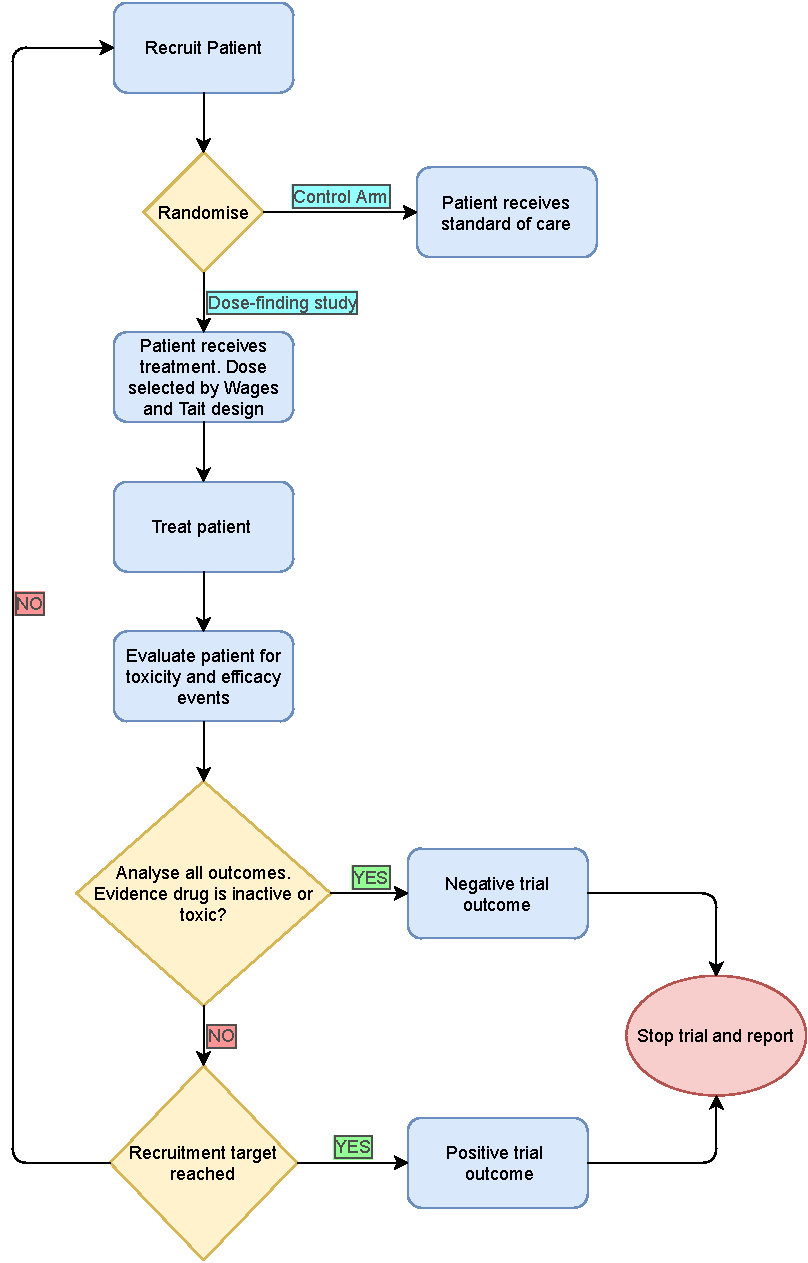
\includegraphics[width=0.77\textwidth]{WT-TwoArmExample}
\end{figure}

There is another approach that could also be used to include a control arm rather than our proposed design RtC-WT. A two-arm randomised design could be used where patients are allocated to either a control arm or a dose-finding arm. Those patients allocated in the dose-finding arm will then be a part of the WT design (see Figure \ref{fig_wt:TwoArmExample}). This approach maintains many of the traditional qualities of a two-arm randomised trial. The number of patients in each arm can be specified this way and we guarantee a minimum number of patients in our control arm. Also, the characteristics of patients in both arms are likely to be similar which would be beneficial when making comparisons between the two arms. A downside of this method is that the data for control patients are no longer included in the modelling process. Whilst control patients may still be observed for efficacious and toxic events these will not be included in the modelling. As such the ability to make inferences on the dose-toxicity and efficacy relationships in reference to a control/ standard of care dose is lost. 

Both of these approaches have their merit but also have flaws as well. RtC-WT is somewhat of a middle ground that aims to recruit patients to a control dose and include the control patients' data in the modelling process all whilst maintaining reasonable operating characteristics. We detail RtC-WT in Section \ref{WT:Design-RtC-WT} and explore the operating characteristics of this design in Section \ref{WT:Evaluation-of-the-Extension}.

%-----------------------------------
%	SUBSECTION 3.2
%-----------------------------------
\subsection{Design of the Proposed Extension RtC-WT}
\label{WT:Design-RtC-WT}

With this extension, much of the Wages and Tait design stays the same. The modification only impacts the adaptive randomisation (AR) phase and requires some additional specifications at the start of the trial. Firstly, we set the lowest dose-level $d_1$ to be the control dose-level. This dose-level should be included in the working models for efficacy and toxicity and should be treated like any other dose-level. Even if toxicity and efficacy events are expected to be non-existent for control, their corresponding skeleton values must be non-zero. Investigators also need to consider a randomisation probability $\phi_R$ for the control dose. During the AR phase, $\phi_R$ represents the probability of selecting the control dose as the next dose level. The probability of randomisation $R_i$ for other dose in $\mathscrsfs{A}_j$ is scaled accordingly such that the $\sum_{d_i \in \mathscrsfs{A}_j} R_i = 1$. The adaptive randomisation probabilities can now be expressed as 

\begin{equation}
	R_1 = \phi_R,
\end{equation}

\begin{equation}
	R_i = (1-\phi_R)\frac{\hat{\pi}_E(d_i)}{\sum_{d_i \in \mathscrsfs{A}_j}\hat{\pi}_E(d_i)}, \; \; i=2,...,I. 
\end{equation}

Compared to Equation \ref{WT:eq_WT-ARprob} the adaptive randomisation probability is fixed to $\phi_R$ at the lowest dose (the control dose) and for all other dose levels in the admissible set $\mathscrsfs{A}_j$ a scaled randomisation probability is calculated. By fixing the probability for the control dose we guarantee a greater chance of patients being allocated to this dose-level. Although estimates of efficacy at the control dose-level $\hat{\pi}_E(d_1)$ do not directly impact its associated randomisation probability, the efficacy data that generated the estimate is still included in the efficacy modelling and impacts probabilities for the remaining dose-levels. Also, by scaling the remaining probabilities of dose-levels in the admissible set we ensure that those doses with high estimates of efficacy maintain their proportional advantage of selection over the other non-control doses.

Some adjustments were made to the stopping rule for safety. The WT design assesses the lower bound of the 95\% binomial confidence interval of DLT rate for the lowest dose to determine whether or not the trial should be stopped. However, with the RtC-WT design since the lowest dose is the control, it makes little sense to surmise treatment is toxic here since none of the patients on control would have received the experimental treatment. It is also likely the trial would never recommend stopping even if the treatment is toxic since patients on control are unlikely to experience excess toxic events. The RtC-WT design stops for safety by checking for excess toxicity at the second-lowest dose-level (the first treatment dose-level).

Once the AR phase ends, dose-levels are no longer selected by adaptive randomisation. At this point, it will be difficult for patients to be recruited to the control dose since recommended doses will be based on those with the greatest estimates of efficacy. As such it is important to consider the values set for both your randomisation probability for control $\phi_R$ and the size of the AR phase $j_R$. Wages and Tait simply suggest a 50:50 split between both the AR phase and the maximisation phase and show relatively good performance at this level. However, for RtC-WT the AR phase is the main component and more thought should be given here. In the next section, we explore multiple combinations to better understand how these choices impact the operating characteristics of the design. We also compare RtC-WT to the two alternative designs mentioned in section  \ref{WT:Rationale-for-RtC-WT} via simulations and the inspection of operating characteristics specifically, the selection probabilities of the OBD and patient allocation numbers at each dose-level. 

%----------------------------------------------------------------------------------------
%	SECTION 4
%----------------------------------------------------------------------------------------
\section{Evaluation and Exploration of the Extension via Simulations}
\label{WT:Evaluation-of-the-Extension}

In this section, we evaluate the performance of RtC-WT in comparison to the two alternative designs mentioned in Section \ref{WT:Rationale-for-RtC-WT}. We also explore the impact of changing the probability of randomisation to control and the number of patients included in the adaptive randomisation phase. These will both be assessed via simulation and inspection of their operating characteristics. To facilitate simulations, a generic trial example will be utilised along with a variety of scenarios. 

%-----------------------------------
%	SUBSECTION 4.1
%-----------------------------------
\subsection{Design Specification}
\label{WT:Design-Spec}

Here we detail the design specifications for RtC-WT that we will be using throughout this section. We assume five dose-levels, where the lowest dose is considered to be the control dose-level. The maximum sample size of the trial is set at 60 with patients recruited in cohorts of three and the first cohort starting at dose-level two (the first treatment dose-level). The pre-specified toxicity upper bound and efficacy lower bound are set at $\phi_T = 0.35$ and $\phi_E = 0.50$ respectively. Toxicity and efficacy skeletons, $p_i$ and $q_i$ respectively, are presented in Table \ref{tab_wt:tox-eff-skeleton}. In terms of efficacy relationships monotonic, unimodal and plateau skeletons were all used. We assume that each of the seven efficacy skeletons is equally likely and set $\upsilon(k) = \frac{1}{7}$. 


\begin{table}[!h]
	\centering
	\caption{Toxicity and efficacy skeletons for RtC-WT in the example trial.}
	\label{tab_wt:tox-eff-skeleton}
	\begin{tabular}{c|ccccc}
		\hline
		\multicolumn{1}{c|}{\multirow{2}{*}{\textbf{Skeleton}}} & \multicolumn{5}{c}{\textbf{Dose-levels}}                       \\
		\multicolumn{1}{c|}{}                                   & \textbf{1} & \textbf{2} & \textbf{3} & \textbf{4} & \textbf{5} \\ \hline
		$p_i$    & 0.1 & 0.15 & 0.25 & 0.35 & 0.45 \\
		$q_{i1}$ & 0.3 & 0.7 & 0.6 & 0.5 & 0.4 \\
		$q_{i2}$ & 0.3 & 0.6 & 0.7 & 0.6 & 0.5 \\
		$q_{i3}$ & 0.3 & 0.5 & 0.6 & 0.7 & 0.6 \\
		$q_{i4}$ & 0.3 & 0.4 & 0.5 & 0.6 & 0.7 \\
		$q_{i5}$ & 0.3 & 0.5 & 0.6 & 0.7 & 0.7 \\
		$q_{i6}$ & 0.3 & 0.6 & 0.7 & 0.7 & 0.7 \\
		$q_{i7}$ & 0.3 & 0.7 & 0.7 & 0.7 & 0.7 \\ \hline
	\end{tabular}
\end{table}

For the control dose, we have set our prior beliefs for the probability of toxicity at 10\% and the probability of efficacy at 30\%. This can of course be adjusted if there is reason to believe that the control dose may be slightly more/less effective or toxic. 

Wages and Tait recommend $(2I-1)$ efficacy skeletons be used which in this example would be nine, however, we have only considered seven. As there are only four active doses and we are assuming we understand the control dose in terms of toxicity and probability then seven different skeletons fits in the Wages and Tait's recommendation. As we are investigating control plus some experimental treatment it is implausible to have scenarios where efficacy falls as dose increases. So, we have removed the two efficacy skeletons with dose-efficacy relationships that suggest the lowest dose would be the most efficacious. For completeness, the first extra skeleton would be unimodal with the highest efficacy occurring at dose-level one (i.e. 0.7, 0.6, 0.5, 0.4, 0.3 for dose-levels 1-5) and the second skeleton would be a plateau relationship with the plateau beginning at dose-level one (i.e. 0.7, 0.7, 0.7, 0.7, 0.7 for dose-levels 1-5). 

We also include the same stopping rules for safety and futility with the safety rule assessing toxicity at dose-level two. A rule will also be implemented to prevent the skipping of untried doses when escalating. This rule does not apply when de-escalating. 

The two parameters we have left to specify are the fixed adaptive randomisation probability for control $\phi_R$ and the number of patients included in the adaptive randomisation phase $j_R$. In Section \ref{WT:Design-RtC-WT} we briefly discussed the importance of giving thought when setting these values. This is due to the fact they are the main factors driving how RtC-WT works compared to the standard WT design. For example, one could set the AR phase to last for the whole trial and keep a relatively low probability to randomise to control. Alternatively, the AR phase can be set for half the patients in the trial and double the probability of randomisation could be used. These two approaches could allocate the same number of patients in the control arm but have different operating characteristics. It could be hypothesised that by setting the AR phase for the whole trial you miss out on the maximisation phase where patients are allocated to the estimated most efficacious dose which could yield slightly worse operating characteristics. We explore different combinations of these parameters in the next section. 


%-----------------------------------
%	SUBSECTION 4.2
%-----------------------------------
\subsection{Impact of AR phase size and probability of randomisation to control on RtC-WT}
\label{WT:Impact-ARandRTCon-RtC-WT}


The effect of adjusting the probability of randomising to control $\phi_R$ is fairly intuitive, as the probability increases the percentage chance that patients are allocated to the control dose-level also increases. However, this is only in isolation without considering the size of the AR phase. Increasing the AR phase would also mean more patients are likely allocated to the control dose-level since the randomisation only occurs in the AR phase. The interest lies within the interaction of both of these components and their impacts on operating characteristics. To gain a better understanding of this impact on RtC-WT we consider multiple combinations. 

We look at two different probabilities for randomisation to control, $\phi_R = 0.2$ and $\phi_R = 0.33$ i.e. 20\% and 33\% probability of patients being allocated to the control dose-level during the AR phase of the trial. We also consider varying AR phase sizes, specifically $j_R = 0, 15, 30, 45 ,60$ essentially looking at when the AR phase lasts 0\%, 25\%, 50\%, 75\% and 100\% of the trial. The inclusion of setting the AR phase as 0 is somewhat counter-intuitive since the trial will just be run using the maximisation phase where the most efficacious doses are allocated. As such it is unlikely that the control dose-level would ever be the most efficacious specifically in our scenario here. However, its inclusion will serve as a benchmark as the design most likely to achieve optimal performance in terms of locating the OBD since there will be no randomisation and the estimated most efficacious dose will always be the one being tested. Similarly, by setting the AR phase at 60 we limit some of the designs features by never entering the maximisation phase to select dose levels based on efficacy. Also, the stopping rule for futility does not come into play. Although, many more combinations could be explored this set provide a good basis for us to gain a better understanding of how RtC-WT works. It also helps us understand how best to optimise RtC-WT for comparisons with alternative designs later on.  

To compare these different combinations we use simulations covering a wide range of scenarios. For each scenario, we simulate 10000 trials each consisting of 60 patients recruited in cohorts of three. Patient outcomes for toxicity and efficacy are randomly sampled using true toxicity and true efficacy probabilities, these are assumed to be independent of each other. Dose-allocation decisions are made after each cohort of patients and then the subsequent cohort is allocated the recommended dose. The trial could also be stopped if the recruitment target is reached or if any of the stopping rules are triggered. The rest of the design specification is as defined in Section \ref{WT:Design-Spec}. 

The true toxicity and efficacy probabilities are manipulated to produce each scenario for the simulations. Table \ref{tab_wt:sim-scenarios} shows a summary of the scenarios that will be used. We look at a combination of five different efficacy curves with three toxicity curves giving 15 scenarios altogether. The five dose-efficacy relationships we consider are; monotonically increasing, unimodal (at dose level 3), plateau (starting at dose level 3), monotonically decreasing and finally no efficacy. For toxicity we look at scenarios where all doses are tolerable, all doses are toxic and a scenario where only higher doses (dose-levels 4 and 5) are toxic. We also list which doses would be considered the OBD under the designs specification along with which doses would be good for each of the scenarios. The OBD in this context would be the dose which maximises efficacy whilst not breaching the toxicity limit. Good doses are those which are considered safe (probability of toxicity $\leq$ 35\%) and efficacious (probability of efficacy $\geq$ 50\%). For scenarios that are too toxic/lack efficacy, we would expect the trial to stop early, here we have labelled the OBD as being the probability of stopping and good doses as the probability of stopping and selecting dose-level 1, the control dose. Whilst allocating patients to dose-level 1 in these scenarios is not necessarily a bad thing it would likely mean more patients are exposed to the toxic/inefficacious doses which is not optimal, hence the distinction.  

Operating characteristics for the scenarios under investigation are given in Table \ref{tab_wt:SelectProbCombos}. The table provides the following operating characteristics: 

\begin{itemize}
	\item P(OBD) - Probability of selecting the OBD
	\item P(Good) - Probability of selecting a good dose
	\item N(OBD) - Mean number of patients treated at the OBD
	\item N(Good) - Mean number of patients treated at good doses
	\item N(Control) - Mean number of patients treated at the control dose (dose-level 1)
\end{itemize}

These are provided for each scenario under the 10 different parameterisations of $\phi_R$ and $j_R$. For certain scenarios, where the ideal outcome would be to stop early, N(OBD) is left blank as patients are not allocated to a specific dose. Also, for these scenarios N(Good) and N(Control) are the same as the only good dose patients can be allocated to is the control. Then for scenarios where there is only one good dose-level that would be the OBD as well so P(OBD) and P(Good) would be the same as would N(OBD) and N(Good). 

\newpage

\begin{table}[h!]
	\centering
	\caption{Summary of the efficacy and toxicity curves used in each scenario.}
	\label{tab_wt:sim-scenarios}
\resizebox{\textwidth}{!}{%
	\begin{tabular}{cc|ccccc|l|cc}
		\hline
		\multicolumn{2}{c|}{\textbf{Scenario}} & \textbf{1} & \textbf{2} & \textbf{3} & \textbf{4} & \textbf{5} & \textbf{Description} & \textbf{OBD} & \textbf{Good Dose} \\ \hline
		\multirow{2}{*}{1} & tox & 0.1 & 0.2 & 0.25 & 0.3 & 0.35 & All doses tolerable & \multirow{2}{*}{5} & \multirow{2}{*}{3-5} \\
		& eff & 0.3 & 0.4 & 0.5 & 0.6 & 0.7 & Monotone increasing &  &  \\ \hline
		\multirow{2}{*}{2} & tox & 0.1 & 0.45 & 0.5 & 0.55 & 0.6 & Too toxic & \multirow{2}{*}{Stop} & \multirow{2}{*}{Stop/Control} \\
		& eff & 0.3 & 0.4 & 0.5 & 0.6 & 0.7 & Monotone increasing &  &  \\ \hline
		\multirow{2}{*}{3} & tox & 0.1 & 0.25 & 0.35 & 0.45 & 0.55 & High doses toxic & \multirow{2}{*}{3} & \multirow{2}{*}{3} \\
		& eff & 0.3 & 0.4 & 0.5 & 0.6 & 0.7 & Monotone increasing &  &  \\ \hline
		\multirow{2}{*}{4} & tox & 0.1 & 0.2 & 0.25 & 0.3 & 0.35 & All doses tolerable & \multirow{2}{*}{3} & \multirow{2}{*}{3-4} \\
		& eff & 0.3 & 0.4 & 0.7 & 0.5 & 0.4 & Unimodal &  &  \\ \hline
		\multirow{2}{*}{5} & tox & 0.1 & 0.45 & 0.5 & 0.55 & 0.6 & Too toxic & \multirow{2}{*}{Stop} & \multirow{2}{*}{Stop/Control} \\
		& eff & 0.3 & 0.4 & 0.7 & 0.5 & 0.4 & Unimodal &  &  \\ \hline
		\multirow{2}{*}{6} & tox & 0.1 & 0.25 & 0.35 & 0.45 & 0.55 & High doses toxic & \multirow{2}{*}{3} & \multirow{2}{*}{3} \\
		& eff & 0.3 & 0.4 & 0.7 & 0.5 & 0.4 & Unimodal &  &  \\ \hline
		\multirow{2}{*}{7} & tox & 0.1 & 0.2 & 0.25 & 0.3 & 0.35 & All doses tolerable & \multirow{2}{*}{3} & \multirow{2}{*}{3-5} \\
		& eff & 0.3 & 0.4 & 0.6 & 0.6 & 0.6 & Plateau &  &  \\ \hline
		\multirow{2}{*}{8} & tox & 0.1 & 0.45 & 0.5 & 0.55 & 0.6 & Too toxic & \multirow{2}{*}{Stop} & \multirow{2}{*}{Stop/Control} \\
		& eff & 0.3 & 0.4 & 0.6 & 0.6 & 0.6 & Plateau &  &  \\ \hline
		\multirow{2}{*}{9} & tox & 0.1 & 0.25 & 0.35 & 0.45 & 0.55 & High doses toxic & \multirow{2}{*}{3} & \multirow{2}{*}{3} \\
		& eff & 0.3 & 0.4 & 0.6 & 0.6 & 0.6 & Plateau &  &  \\ \hline
		\multirow{2}{*}{10} & tox & 0.1 & 0.2 & 0.25 & 0.3 & 0.35 & All doses tolerable & \multirow{2}{*}{2} & \multirow{2}{*}{2-4} \\
		& eff & 0.3 & 0.7 & 0.6 & 0.5 & 0.4 & Monotone decreasing &  &  \\ \hline
		\multirow{2}{*}{11} & tox & 0.1 & 0.45 & 0.5 & 0.55 & 0.6 & Too toxic & \multirow{2}{*}{Stop} & \multirow{2}{*}{Stop/Control} \\
		& eff & 0.3 & 0.7 & 0.6 & 0.5 & 0.4 & Monotone decreasing &  &  \\ \hline
		\multirow{2}{*}{12} & tox & 0.1 & 0.25 & 0.35 & 0.45 & 0.55 & High doses toxic & \multirow{2}{*}{2} & \multirow{2}{*}{2-3} \\
		& eff & 0.3 & 0.7 & 0.6 & 0.5 & 0.4 & Monotone decreasing &  &  \\ \hline
		\multirow{2}{*}{13} & tox & 0.1 & 0.2 & 0.25 & 0.3 & 0.35 & All doses tolerable & \multirow{2}{*}{Stop} & \multirow{2}{*}{Stop/Control} \\
		& eff & 0.3 & 0.3 & 0.3 & 0.3 & 0.3 & No Efficacy &  &  \\ \hline
		\multirow{2}{*}{14} & tox & 0.1 & 0.45 & 0.5 & 0.55 & 0.6 & Too toxic & \multirow{2}{*}{Stop} & \multirow{2}{*}{Stop/Control} \\
		& eff & 0.3 & 0.3 & 0.3 & 0.3 & 0.3 & No Efficacy &  &  \\ \hline
		\multirow{2}{*}{15} & tox & 0.1 & 0.25 & 0.35 & 0.45 & 0.55 & High doses toxic & \multirow{2}{*}{Stop} & \multirow{2}{*}{Stop/Control} \\
		& eff & 0.3 & 0.3 & 0.3 & 0.3 & 0.3 & No Efficacy &  &  \\ \hline
	\end{tabular}%
}
\end{table}

\newpage

\setlength\LTcapwidth{\textwidth}
\begingroup\fontsize{9}{11}\selectfont

\begin{longtable}[h!]{cccccccccc}
		
	\caption[Operating characteristics for multiple combinations of parameters.]{\label{tab_wt:SelectProbCombos}Operating characteristics for multiple combinations of AR phase size and probabilities for randomisation to control. Probability of selecting the OBD or good dose levels, mean number of patients treated at those dose levels and at the control dose after 10000 simulations.}\\
	\toprule
	Scenario & $\phi_R$ & $j_R$ & OBD & Good Doses & P(OBD) & P(Good) & N(OBD) & N(Good) & N(Control)\\
	\midrule
	\endfirsthead
	\caption[]{Operating characteristics (continued)}\\
	\toprule
	Scenario & \ $\phi_R$ & $j_R$ & OBD & Good Doses & P(OBD) & P(Good) & N(OBD) & N(Good) & N(Control)\\
	\midrule
	\endhead
	
	\endfoot
	\bottomrule
	\endlastfoot
 &  & 0 & 5 & 3-5 & 0.05 & 0.60 & 2.8 & 32.1 & 1.2\\
\nopagebreak
&  & 15 & 5 & 3-5 & 0.05 & 0.65 & 2.7 & 32 & 3.6\\
\nopagebreak
&  & 30 & 5 & 3-5 & 0.05 & 0.71 & 2.2 & 31.1 & 6.4\\
\nopagebreak
&  & 45 & 5 & 3-5 & 0.05 & 0.76 & 1.5 & 27.5 & 9.4\\
\nopagebreak
& \multirow{-5}{*}{\centering\arraybackslash 0.2} & 60 & 5 & 3-5 & 0.04 & 0.80 & 1.1 & 22.9 & 12.4\\
\nopagebreak
&  & 0 & 5 & 3-5 & 0.05 & 0.60 & 2.8 & 32.1 & 1.2\\
\nopagebreak
&  & 15 & 5 & 3-5 & 0.07 & 0.67 & 3.1 & 32.6 & 4.9\\
\nopagebreak
&  & 30 & 5 & 3-5 & 0.06 & 0.75 & 2.2 & 30.4 & 9.8\\
\nopagebreak
&  & 45 & 5 & 3-5 & 0.05 & 0.79 & 1.3 & 25.5 & 14.7\\
\nopagebreak
\multirow{-10}{*}{\centering\arraybackslash 1} & \multirow{-5}{*}{\centering\arraybackslash 0.33} & 60 & 5 & 3-5 & 0.03 & 0.82 & 0.8 & 19.4 & 19.6\\
\cmidrule{1-10}\pagebreak[0]
&  & 0 & stop & stop/1 & 0.81 & 0.85 & - & 10.1 & 10.1\\
\nopagebreak
&  & 15 & stop & stop/1 & 0.80 & 0.85 & - & 11 & 11\\
\nopagebreak
&  & 30 & stop & stop/1 & 0.77 & 0.81 & - & 13.2 & 13.2\\
\nopagebreak
&  & 45 & stop & stop/1 & 0.72 & 0.75 & - & 15.6 & 15.6\\
\nopagebreak
& \multirow{-5}{*}{\centering\arraybackslash 0.2} & 60 & stop & stop/1 & 0.41 & 0.50 & - & 17.9 & 17.9\\
\nopagebreak
&  & 0 & stop & stop/1 & 0.81 & 0.85 & - & 10.1 & 10.1\\
\nopagebreak
&  & 15 & stop & stop/1 & 0.77 & 0.83 & - & 11.4 & 11.4\\
\nopagebreak
&  & 30 & stop & stop/1 & 0.75 & 0.79 & - & 14 & 14\\
\nopagebreak
&  & 45 & stop & stop/1 & 0.67 & 0.70 & - & 17.6 & 17.6\\
\nopagebreak
\multirow{-10}{*}{\centering\arraybackslash 2} & \multirow{-5}{*}{\centering\arraybackslash 0.33} & 60 & stop & stop/1 & 0.38 & 0.42 & - & 20.7 & 20.7\\
\cmidrule{1-10}\pagebreak[0]
&  & 0 & 3 & 3 & 0.25 & 0.25 & 15.5 & 15.5 & 2.6\\
\nopagebreak
&  & 15 & 3 & 3 & 0.31 & 0.31 & 16.8 & 16.8 & 4.7\\
\nopagebreak
&  & 30 & 3 & 3 & 0.35 & 0.35 & 16.8 & 16.8 & 7.5\\
\nopagebreak
&  & 45 & 3 & 3 & 0.42 & 0.42 & 15.5 & 15.5 & 10.4\\
\nopagebreak
& \multirow{-5}{*}{\centering\arraybackslash 0.2} & 60 & 3 & 3 & 0.48 & 0.48 & 12.7 & 12.7 & 13.3\\
\nopagebreak
&  & 0 & 3 & 3 & 0.25 & 0.25 & 15.5 & 15.5 & 2.6\\
\nopagebreak
&  & 15 & 3 & 3 & 0.32 & 0.32 & 17.2 & 17.2 & 5.8\\
\nopagebreak
&  & 30 & 3 & 3 & 0.39 & 0.39 & 17.3 & 17.3 & 10.4\\
\nopagebreak
&  & 45 & 3 & 3 & 0.46 & 0.46 & 15.2 & 15.2 & 15.2\\
\nopagebreak
\multirow{-10}{*}{\centering\arraybackslash 3} & \multirow{-5}{*}{\centering\arraybackslash 0.33} & 60 & 3 & 3 & 0.52 & 0.52 & 11.5 & 11.5 & 20.1\\
\cmidrule{1-10}\pagebreak[0]
&  & 0 & 3 & 3-4 & 0.69 & 0.75 & 32.3 & 37.2 & 1.3\\
\nopagebreak
&  & 15 & 3 & 3-4 & 0.69 & 0.76 & 30.3 & 35.5 & 3.5\\
\nopagebreak
&  & 30 & 3 & 3-4 & 0.71 & 0.81 & 26.4 & 32.3 & 6.5\\
\nopagebreak
&  & 45 & 3 & 3-4 & 0.73 & 0.83 & 21.6 & 27.4 & 9.5\\
\nopagebreak
& \multirow{-5}{*}{\centering\arraybackslash 0.2} & 60 & 3 & 3-4 & 0.71 & 0.83 & 16 & 21.7 & 12.4\\
\nopagebreak
&  & 0 & 3 & 3-4 & 0.69 & 0.75 & 32.3 & 37.2 & 1.3\\
\nopagebreak
&  & 15 & 3 & 3-4 & 0.69 & 0.77 & 29.5 & 35.1 & 5\\
\nopagebreak
&  & 30 & 3 & 3-4 & 0.70 & 0.81 & 24.8 & 31 & 9.9\\
\nopagebreak
&  & 45 & 3 & 3-4 & 0.70 & 0.84 & 19.7 & 25.4 & 14.7\\
\nopagebreak
\multirow{-10}{*}{\centering\arraybackslash 4} & \multirow{-5}{*}{\centering\arraybackslash 0.33} & 60 & 3 & 3-4 & 0.68 & 0.83 & 13.7 & 18.5 & 19.5\\
\cmidrule{1-10}\pagebreak[0]
&  & 0 & stop & stop/1 & 0.81 & 0.86 & - & 10.1 & 10.1\\
\nopagebreak
&  & 15 & stop & stop/1 & 0.79 & 0.84 & - & 11.1 & 11.1\\
\nopagebreak
&  & 30 & stop & stop/1 & 0.77 & 0.82 & - & 13.1 & 13.1\\
\nopagebreak
&  & 45 & stop & stop/1 & 0.71 & 0.75 & - & 15.6 & 15.6\\
\nopagebreak
& \multirow{-5}{*}{\centering\arraybackslash 0.2} & 60 & stop & stop/1 & 0.41 & 0.49 & - & 17.9 & 17.9\\
\nopagebreak
&  & 0 & stop & stop/1 & 0.81 & 0.86 & - & 10.1 & 10.1\\
\nopagebreak
&  & 15 & stop & stop/1 & 0.78 & 0.83 & - & 11.3 & 11.3\\
\nopagebreak
&  & 30 & stop & stop/1 & 0.75 & 0.78 & - & 14.1 & 14.1\\
\nopagebreak
&  & 45 & stop & stop/1 & 0.67 & 0.70 & - & 17.6 & 17.6\\
\nopagebreak
\multirow{-10}{*}{\centering\arraybackslash 5} & \multirow{-5}{*}{\centering\arraybackslash 0.33} & 60 & stop & stop/1 & 0.38 & 0.43 & - & 20.8 & 20.8\\
\cmidrule{1-10}\pagebreak[0]
&  & 0 & 3 & 3 & 0.37 & 0.37 & 21.2 & 21.2 & 2.6\\
\nopagebreak
&  & 15 & 3 & 3 & 0.41 & 0.41 & 21.3 & 21.3 & 4.5\\
\nopagebreak
&  & 30 & 3 & 3 & 0.45 & 0.45 & 19.6 & 19.6 & 7.5\\
\nopagebreak
&  & 45 & 3 & 3 & 0.50 & 0.50 & 17.1 & 17.1 & 10.4\\
\nopagebreak
& \multirow{-5}{*}{\centering\arraybackslash 0.2} & 60 & 3 & 3 & 0.54 & 0.54 & 12.8 & 12.8 & 13.4\\
\nopagebreak
&  & 0 & 3 & 3 & 0.37 & 0.37 & 21.2 & 21.2 & 2.6\\
\nopagebreak
&  & 15 & 3 & 3 & 0.42 & 0.42 & 21.4 & 21.4 & 5.8\\
\nopagebreak
&  & 30 & 3 & 3 & 0.50 & 0.50 & 20.3 & 20.3 & 10.4\\
\nopagebreak
&  & 45 & 3 & 3 & 0.55 & 0.55 & 16.6 & 16.6 & 15.1\\
\nopagebreak
\multirow{-10}{*}{\centering\arraybackslash 6} & \multirow{-5}{*}{\centering\arraybackslash 0.33} & 60 & 3 & 3 & 0.59 & 0.59 & 11.5 & 11.5 & 20.1\\
\cmidrule{1-10}\pagebreak[0]
&  & 0 & 3 & 3-5 & 0.48 & 0.70 & 23.9 & 35.6 & 1.3\\
\nopagebreak
&  & 15 & 3 & 3-5 & 0.50 & 0.73 & 23.7 & 35 & 3.5\\
\nopagebreak
&  & 30 & 3 & 3-5 & 0.52 & 0.78 & 21.8 & 32.4 & 6.4\\
\nopagebreak
&  & 45 & 3 & 3-5 & 0.56 & 0.81 & 19.3 & 27.9 & 9.4\\
\nopagebreak
& \multirow{-5}{*}{\centering\arraybackslash 0.2} & 60 & 3 & 3-5 & 0.57 & 0.82 & 15.8 & 22.5 & 12.5\\
\nopagebreak
&  & 0 & 3 & 3-5 & 0.48 & 0.70 & 23.9 & 35.6 & 1.3\\
\nopagebreak
&  & 15 & 3 & 3-5 & 0.49 & 0.75 & 22.7 & 35.1 & 5\\
\nopagebreak
&  & 30 & 3 & 3-5 & 0.51 & 0.80 & 20.8 & 31.6 & 9.7\\
\nopagebreak
&  & 45 & 3 & 3-5 & 0.55 & 0.84 & 17.7 & 26 & 14.7\\
\nopagebreak
\multirow{-10}{*}{\centering\arraybackslash 7} & \multirow{-5}{*}{\centering\arraybackslash 0.33} & 60 & 3 & 3-5 & 0.56 & 0.84 & 13.7 & 19.6 & 19.5\\
\cmidrule{1-10}\pagebreak[0]
&  & 0 & stop & stop/1 & 0.81 & 0.85 & - & 10.2 & 10.2\\
\nopagebreak
&  & 15 & stop & stop/1 & 0.79 & 0.84 & - & 11.1 & 11.1\\
\nopagebreak
&  & 30 & stop & stop/1 & 0.77 & 0.81 & - & 13.2 & 13.2\\
\nopagebreak
&  & 45 & stop & stop/1 & 0.71 & 0.76 & - & 15.6 & 15.6\\
\nopagebreak
& \multirow{-5}{*}{\centering\arraybackslash 0.2} & 60 & stop & stop/1 & 0.41 & 0.50 & - & 17.9 & 17.9\\
\nopagebreak
&  & 0 & stop & stop/1 & 0.81 & 0.85 & - & 10.2 & 10.2\\
\nopagebreak
&  & 15 & stop & stop/1 & 0.78 & 0.82 & - & 11.3 & 11.3\\
\nopagebreak
&  & 30 & stop & stop/1 & 0.75 & 0.79 & - & 14 & 14\\
\nopagebreak
&  & 45 & stop & stop/1 & 0.69 & 0.71 & - & 17.4 & 17.4\\
\nopagebreak
\multirow{-10}{*}{\centering\arraybackslash 8} & \multirow{-5}{*}{\centering\arraybackslash 0.33} & 60 & stop & stop/1 & 0.38 & 0.43 & - & 20.8 & 20.8\\
\cmidrule{1-10}\pagebreak[0]
&  & 0 & 3 & 3 & 0.34 & 0.34 & 18.6 & 18.6 & 2.6\\
\nopagebreak
&  & 15 & 3 & 3 & 0.36 & 0.36 & 19.2 & 19.2 & 4.6\\
\nopagebreak
&  & 30 & 3 & 3 & 0.42 & 0.42 & 18.3 & 18.3 & 7.5\\
\nopagebreak
&  & 45 & 3 & 3 & 0.45 & 0.45 & 16.3 & 16.3 & 10.3\\
\nopagebreak
& \multirow{-5}{*}{\centering\arraybackslash 0.2} & 60 & 3 & 3 & 0.50 & 0.50 & 12.9 & 12.9 & 13.3\\
\nopagebreak
&  & 0 & 3 & 3 & 0.34 & 0.34 & 18.6 & 18.6 & 2.6\\
\nopagebreak
&  & 15 & 3 & 3 & 0.38 & 0.38 & 19.7 & 19.7 & 5.9\\
\nopagebreak
&  & 30 & 3 & 3 & 0.45 & 0.45 & 18.6 & 18.6 & 10.4\\
\nopagebreak
&  & 45 & 3 & 3 & 0.52 & 0.52 & 15.9 & 15.9 & 15.2\\
\nopagebreak
\multirow{-10}{*}{\centering\arraybackslash 9} & \multirow{-5}{*}{\centering\arraybackslash 0.33} & 60 & 3 & 3 & 0.56 & 0.56 & 11.5 & 11.5 & 20.1\\
\cmidrule{1-10}\pagebreak[0]
&  & 0 & 2 & 2-4 & 0.77 & 0.97 & 45.1 & 57.1 & 1.3\\
\nopagebreak
&  & 15 & 2 & 2-4 & 0.79 & 0.97 & 41.8 & 55.3 & 3.5\\
\nopagebreak
&  & 30 & 2 & 2-4 & 0.79 & 0.98 & 37.2 & 52.5 & 6.5\\
\nopagebreak
&  & 45 & 2 & 2-4 & 0.79 & 0.99 & 32.2 & 49.6 & 9.4\\
\nopagebreak
& \multirow{-5}{*}{\centering\arraybackslash 0.2} & 60 & 2 & 2-4 & 0.80 & 0.99 & 26.4 & 46.4 & 12.3\\
\nopagebreak
&  & 0 & 2 & 2-4 & 0.77 & 0.97 & 45.1 & 57.1 & 1.3\\
\nopagebreak
&  & 15 & 2 & 2-4 & 0.77 & 0.97 & 40.1 & 53.6 & 5\\
\nopagebreak
&  & 30 & 2 & 2-4 & 0.76 & 0.98 & 34.6 & 49.1 & 9.8\\
\nopagebreak
&  & 45 & 2 & 2-4 & 0.76 & 0.99 & 28.4 & 44.3 & 14.7\\
\nopagebreak
\multirow{-10}{*}{\centering\arraybackslash 10} & \multirow{-5}{*}{\centering\arraybackslash 0.33} & 60 & 2 & 2-4 & 0.78 & 0.99 & 22.3 & 39.2 & 19.6\\
\cmidrule{1-10}\pagebreak[0]
&  & 0 & stop & stop/1 & 0.65 & 0.74 & - & 11.7 & 11.7\\
\nopagebreak
&  & 15 & stop & stop/1 & 0.65 & 0.72 & - & 12.3 & 12.3\\
\nopagebreak
&  & 30 & stop & stop/1 & 0.62 & 0.69 & - & 13.8 & 13.8\\
\nopagebreak
&  & 45 & stop & stop/1 & 0.57 & 0.63 & - & 15.7 & 15.7\\
\nopagebreak
& \multirow{-5}{*}{\centering\arraybackslash 0.2} & 60 & stop & stop/1 & 0.41 & 0.49 & - & 17.9 & 17.9\\
\nopagebreak
&  & 0 & stop & stop/1 & 0.65 & 0.74 & - & 11.7 & 11.7\\
\nopagebreak
&  & 15 & stop & stop/1 & 0.64 & 0.72 & - & 12.5 & 12.5\\
\nopagebreak
&  & 30 & stop & stop/1 & 0.60 & 0.67 & - & 14.7 & 14.7\\
\nopagebreak
&  & 45 & stop & stop/1 & 0.52 & 0.56 & - & 17.7 & 17.7\\
\nopagebreak
\multirow{-10}{*}{\centering\arraybackslash 11} & \multirow{-5}{*}{\centering\arraybackslash 0.33} & 60 & stop & stop/1 & 0.38 & 0.42 & - & 20.9 & 20.9\\
\cmidrule{1-10}\pagebreak[0]
&  & 0 & 2 & 2-3 & 0.83 & 0.92 & 47.3 & 53.7 & 2.7\\
\nopagebreak
&  & 15 & 2 & 2-3 & 0.83 & 0.93 & 43.6 & 51.8 & 4.7\\
\nopagebreak
&  & 30 & 2 & 2-3 & 0.82 & 0.95 & 39.7 & 49.3 & 7.4\\
\nopagebreak
&  & 45 & 2 & 2-3 & 0.84 & 0.96 & 35.9 & 46.4 & 10.4\\
\nopagebreak
& \multirow{-5}{*}{\centering\arraybackslash 0.2} & 60 & 2 & 2-3 & 0.85 & 0.97 & 31.7 & 43.5 & 13.2\\
\nopagebreak
&  & 0 & 2 & 2-3 & 0.83 & 0.92 & 47.3 & 53.7 & 2.7\\
\nopagebreak
&  & 15 & 2 & 2-3 & 0.81 & 0.94 & 41.9 & 50.7 & 5.9\\
\nopagebreak
&  & 30 & 2 & 2-3 & 0.80 & 0.95 & 36.6 & 46.3 & 10.4\\
\nopagebreak
&  & 45 & 2 & 2-3 & 0.81 & 0.96 & 31.7 & 41.8 & 15.3\\
\nopagebreak
\multirow{-10}{*}{\centering\arraybackslash 12} & \multirow{-5}{*}{\centering\arraybackslash 0.33} & 60 & 2 & 2-3 & 0.82 & 0.97 & 26 & 36.8 & 20\\
\cmidrule{1-10}\pagebreak[0]
&  & 0 & stop & stop/1 & 0.82 & 0.82 & - & 1.2 & 1.2\\
\nopagebreak
&  & 15 & stop & stop/1 & 0.78 & 0.78 & - & 3.5 & 3.5\\
\nopagebreak
&  & 30 & stop & stop/1 & 0.70 & 0.70 & - & 6.5 & 6.5\\
\nopagebreak
&  & 45 & stop & stop/1 & 0.57 & 0.57 & - & 9.5 & 9.5\\
\nopagebreak
& \multirow{-5}{*}{\centering\arraybackslash 0.2} & 60 & stop & stop/1 & 0.01 & 0.01 & - & 12.4 & 12.4\\
\nopagebreak
&  & 0 & stop & stop/1 & 0.82 & 0.82 & - & 1.2 & 1.2\\
\nopagebreak
&  & 15 & stop & stop/1 & 0.76 & 0.76 & - & 4.9 & 4.9\\
\nopagebreak
&  & 30 & stop & stop/1 & 0.68 & 0.68 & - & 9.7 & 9.7\\
\nopagebreak
&  & 45 & stop & stop/1 & 0.54 & 0.54 & - & 14.7 & 14.7\\
\nopagebreak
\multirow{-10}{*}{\centering\arraybackslash 13} & \multirow{-5}{*}{\centering\arraybackslash 0.33} & 60 & stop & stop/1 & 0.01 & 0.01 & - & 19.6 & 19.6\\
\cmidrule{1-10}\pagebreak[0]
&  & 0 & stop & stop/1 & 0.96 & 0.97 & - & 8.3 & 8.3\\
\nopagebreak
&  & 15 & stop & stop/1 & 0.95 & 0.96 & - & 9.6 & 9.6\\
\nopagebreak
&  & 30 & stop & stop/1 & 0.94 & 0.95 & - & 12.4 & 12.4\\
\nopagebreak
&  & 45 & stop & stop/1 & 0.92 & 0.93 & - & 15.5 & 15.5\\
\nopagebreak
& \multirow{-5}{*}{\centering\arraybackslash 0.2} & 60 & stop & stop/1 & 0.42 & 0.50 & - & 17.7 & 17.7\\
\nopagebreak
&  & 0 & stop & stop/1 & 0.96 & 0.97 & - & 8.3 & 8.3\\
\nopagebreak
&  & 15 & stop & stop/1 & 0.95 & 0.96 & - & 9.9 & 9.9\\
\nopagebreak
&  & 30 & stop & stop/1 & 0.93 & 0.94 & - & 13.5 & 13.5\\
\nopagebreak
&  & 45 & stop & stop/1 & 0.89 & 0.90 & - & 17.3 & 17.3\\
\nopagebreak
\multirow{-10}{*}{\centering\arraybackslash 14} & \multirow{-5}{*}{\centering\arraybackslash 0.33} & 60 & stop & stop/1 & 0.38 & 0.43 & - & 20.8 & 20.8\\
\cmidrule{1-10}\pagebreak[0]
&  & 0 & stop & stop/1 & 0.89 & 0.89 & - & 2.3 & 2.3\\
\nopagebreak
&  & 15 & stop & stop/1 & 0.87 & 0.87 & - & 4.5 & 4.5\\
\nopagebreak
&  & 30 & stop & stop/1 & 0.82 & 0.82 & - & 7.3 & 7.3\\
\nopagebreak
&  & 45 & stop & stop/1 & 0.73 & 0.73 & - & 10.4 & 10.4\\
\nopagebreak
& \multirow{-5}{*}{\centering\arraybackslash 0.2} & 60 & stop & stop/1 & 0.02 & 0.03 & - & 13.4 & 13.4\\
\nopagebreak
&  & 0 & stop & stop/1 & 0.89 & 0.89 & - & 2.3 & 2.3\\
\nopagebreak
&  & 15 & stop & stop/1 & 0.86 & 0.86 & - & 5.7 & 5.7\\
\nopagebreak
&  & 30 & stop & stop/1 & 0.80 & 0.80 & - & 10.3 & 10.3\\
\nopagebreak
&  & 45 & stop & stop/1 & 0.69 & 0.70 & - & 15.2 & 15.2\\
\nopagebreak
\multirow{-10}{*}{\centering\arraybackslash 15} & \multirow{-5}{*}{\centering\arraybackslash 0.33} & 60 & stop & stop/1 & 0.02 & 0.03 & - & 20.1 & 20.1\\*
\end{longtable}
\endgroup{}

\newpage

For scenario 1 it is relatively simple to select an admissible dose since all doses are tolerable and efficacy increases monotonically. The difficulty is locating the OBD. All of these combinations fail to identify the OBD (dose-level 5) more than 7\% of the time. Whereas the probability of selecting a good dose is between 60 and 82\%. As the size of the AR phase increases from 0 to 60 so do the selection probabilities for a good dose, going from 60\% to 80\% and 60\% to 82\% for randomisation probabilities of 0.2 and 0.33 respectively. It should be noted that the two designs with no AR phase are identical since the randomisation probabilities are never used. In terms of the number of patients treated we see more patients in the control arm as AR phase size and randomisation probability increase. This is expected since if you increase the amount of time available for cohorts to be randomised or the probability in which that is done, more patients will be recruited to control. By increasing the probability of randomising to control we can also see that fewer patients are being treated at good doses at higher AR sizes. Also, the $\phi_R$ figure does not guarantee that exact percentage of patients in the control dose will be allocated to control but for this scenario, it appears to be somewhat accurate. 

Scenario 2 has no OBD as all treatment doses are considered toxic. For most of the combinations, stopping occurs 67-81\% of the time and including allocation to the control arm we see this increase to 70-85\%. Slightly concerning is the case where the AR phase lasts the whole trial. Here stopping is less frequent at 50\% and 42\% for probabilities of randomisation to control of $\phi_R = 0.2$ and $\phi_R = 0.33$ respectively. To understand why this was occurring we investigated the failure mechanism in individual simulation runs. We found that the design was stopping appropriately for excess toxicity. However, due to setting the AR phase at 60 the maximisation phase never starts and thus the stopping rule for futility never triggers. This is why this parametrisation performs worse comparatively. Even though this scenario is to check for excess toxicity the true efficacy rates used in this scenario could also potentially trigger the futility rule as they are set at 40\% and 50\% for dose-levels 2 and 3. To confirm this we ran some of the parametrisations where the AR size is less than 60 using a design without the futility rule and observed similar stopping rates of 40\% in this scenario. This indicates that overall our design is not that great at stopping for potential toxicities. This could be improved by utilising different stopping criteria. We also observe this difference in scenarios 5, 8, 11 and 14 where we should also be stopping for excess toxicity. The results for $j_R$ = 60 in these scenarios could be interpreted as our baseline for stopping for excess toxicity and the increase stopping in other parametrisations represent how often the futility rule is triggered.      

In scenario 3, the treatment is toxic at high doses and ineffective at lower doses meaning only one dose can be considered good or the OBD. This is a difficult scenario since only one of the five dose-levels is suitable to allocate patients to. The selection probabilities range from 25\% to 52\%. We see as $j_R$ increases selection probabilities also increase. As those designs with smaller AR phases go into the maximisation phase they would be selecting dose-levels based on those in the admissible set with higher efficacy. Since the doses with higher efficacy also have a high toxicity rate there is a chance early on in the trial this is not detected resulting in toxicities at the higher dose-levels causing the trial to stop early. This could be a reason why the designs with the larger AR phase perform better as doses would be randomly selected. This means there is more chance for the lower dose-levels to be chosen and since those are not toxic and the futility rule does not kick in until the maximisation phase there is a higher chance that the OBD can be found.

Scenarios 4-6 look at a unimodal dose-efficacy relationship where efficacy peaks at dose-level 3, with the three same dose-toxicity relationships as before: tolerable, toxic and toxic at high doses for each scenario respectively. Firstly, in scenario 4 we see good performance from all the parametrisations with the probability of selecting the OBD ranging between 68\% and 73\% and the probability of selecting a good dose ranging from 75\% to 84\%. We also see an appropriate amount of patients in the control arm for each of our parameter combinations. An important characteristic of this design to note is the ratio of patients allocated to the control arm compared to the OBD or the good doses. For the higher randomisation probability and maximum AR phase, we can see close to a  1:1 (18.5 at good dose levels to 19.5 at control) allocation between patients treated at control and the best doses. For $\phi_R$ = 0.2, and $j_R$ = 45 we can see close to a 2:1 allocation between those treated at the OBD (21.6) and those treated at the control (9.5). 

Scenario 5 is where treatment is too toxic. Like scenario 2 we see high probabilities of stopping 67\%-81\% and even higher probabilities for stopping and including patients in the control arm (P(Good)) 70\%-86\%. Similarly, the design with an AR phase of 60 performs poorly here and the number of patients allocated to the control is also comparable. 

Scenario 6 only has one good dose to select, making it similar to scenario 3 except with a unimodal efficacy curve. Here, selection probabilities are slightly better ranging from 37\%-59\%. In this scenario, we also observe that the larger the AR phase the greater the selection probability of the OBD. The unimodal efficacy curve means that the dose we want to select is also the dose with the highest efficacy making it easier for the model to pick out. 

A plateau relationship where dose-efficacy stops increasing after dose 3 is looked at in scenarios 7-9 with the three different toxicity curves. In scenario 7 the probability of selecting the OBD ranges from 48\%-56\%, with the probability of selecting a good dose ranging from 70-84\%. In this instance, we see quite a bit of discrepancy going from selecting the OBD to selecting the good doses in terms of the selection probabilities being much higher for good doses. Here we have three doses with the same efficacy level, two of which only have a slight increase in toxicity, which is still below the pre-specified target level. This can also be seen in the number of patients being treated at the good dose versus at the OBD. Scenario 8 exhibits the same behaviour as the other toxic scenarios 2 and 5. Then with scenario 9, the designs also behave similarly to scenarios 3 and 6 where higher dose-levels are too toxic. Selection probabilities range from 34\% to 56\% with the designs with higher AR phases performing better. 

For scenarios 10-12 we look at a monotone decreasing efficacy curve where dose-level 2 is the most efficacious for each of the toxicity curves. In scenario 10 we see very high probabilities of selecting the OBD 76\%-80\% with the probability of selecting a good dose being 97\% or higher. We can also see that in terms of the numbers treated at the OBD and the good doses as these values are relatively high compared to other scenarios. As the OBD is one of the lower dose-levels it makes it relatively easy for the model to select since it is more likely that patients will be allocated there early on into recruitment. Once the maximisation phase starts there would be a lot of efficacy data for that dose and it would be favoured by the model. Even in the cases with larger AR phases, the adaptive randomisation probabilities are still scaled based on efficacy, so it would be more likely they would be allocated to dose-level 2 as well. 

In terms of stopping early if the dose-levels are too toxic for this efficacy curve (scenario 11), performance appears to be worse compared to other too-toxic scenarios (scenarios 2,5,8 and 14). Even so, we still see the same patterns where when the AR phase is 60, the same size as the trial stopping is relatively even worse. Ignoring those designs the stopping probability ranges from 52\%-65\%, adding in the percentage of patients allocated to the control arm this increases to 56\%-74\%. One reason why this may be worse is due to the very high efficacy rates early on and the toxicity rate only being slightly above our target rate by 5\%. Early on into the trial, that 5\% would be difficult for the model to detect but the high efficacy rate is likely to lead to more events so the trial would be less likely to stop until it went to higher dose-levels. Additionally, as the efficacy rates are so high as well for early doses the futility rule is less likely to be triggered meaning less stopping overall compared to other toxic scenarios.  

Typically, the scenarios where the higher doses are more toxic have been the most difficult for the design to deal with. However for scenario 12, with the monotone decreasing efficacy curve we see probabilities of selecting the OBD range from 80\%-85\%. This is even higher than the selection probabilities in scenario 10. However, when we look at the probabilities of selecting good doses (92\%-97\%), whilst still very high it is still slightly less than in scenario 10 where there was one more dose that could be considered good. 

Finally, the last efficacy curve we look at is one where no efficacy is apparent, so efficacy stays at the same level as the control dose. Ideally, in all these scenarios (13-15) we would stop for lack of efficacy. One thing to point out is that the rule for stopping for futility only triggers in the maximisation phase. So, for the designs where $j_R$ = 60 stopping for lack of efficacy will not occur. For scenario 13 we have doses that are all tolerable and can see stopping probabilities ranging from 54\% to 82\%. The only reason to stop in this scenario is for lack of efficacy and so those designs with larger AR phases will not be able to do this until later on into the trial meaning they are less likely to stop as reflected in the stopping probabilities. In terms of selecting the good dose, this is identical to selecting the OBD. So, in this scenario, the control dose is seldom selected as the OBD, even though patients are still being allocated to that dose-level. As stated for an AR phase size of 60 the trial ca not be stopped for futility, so the probability of stopping is due to toxicity. In scenario 14, all the dose-levels are toxic, here we have very high stopping rates between 89\%-96\% except in the case when the AR phase is 60. Scenario 15, where only the higher doses are too toxic stops most of the time as well given a reasonable AR phase between 69\% and 89\% of the time. Again, very rarely is the control dose selected as the OBD. 

Table \ref{tab_wt:OCsCombosSummary} provides a summary of the selection probabilities of the OBD and good doses respectively for all 15 scenarios and 10 parameter combinations. The mean provides a rudimentary glance across the 15 scenarios of how well it selects the OBD / good dose-levels. The standard deviation is a representation of the variability of performance across the different designs. The lower the standard deviation the more homogenous the performance. These statistics have been calculated for all scenarios and then for 'Non-Stopping' scenarios, which are just the scenarios where stopping early for toxicity/futility is not the ideal outcome i.e. scenarios 1,3,4,6,7,9,10 and 12. 

The means for selecting a good dose are about 10\% higher and appear to be slightly less variable. This is to be expected as when selecting the good dose-levels we are allowing for a wider range of doses to be included. There appear to be limited differences between the various parameterisations, except for in the case of when $j_R$ = 60 where its performance is poor in scenarios that require stopping. There are only 1-2 percentage points difference in the mean selection of the OBD and good dose-levels for the various designs. 

\begin{table}[h!]

	\caption[Summary of operating characteristics of multiple combinations and parameters]{\label{tab_wt:OCsCombosSummary}Probabilities of selecting the OBD and good dose levels for multiple combinations of AR phase size and probabilities for randomisation to control, plus summary statistics.}
	\centering
	\resizebox{\linewidth}{!}{
		\begin{tabular}[t]{ccccccccccccccccccccc}
			\toprule
			\multicolumn{2}{c}{ } & \multicolumn{15}{c}{Probability of selecting good dose levels: Scenarios 1-15} & \multicolumn{2}{c}{All scenarios} & \multicolumn{2}{c}{Non Stopping} \\
			\cmidrule(l{3pt}r{3pt}){3-17} \cmidrule(l{3pt}r{3pt}){18-19} \cmidrule(l{3pt}r{3pt}){20-21}
			$\phi_R$ & $j_R$ & 1 & 2 & 3 & 4 & 5 & 6 & 7 & 8 & 9 & 10 & 11 & 12 & 13 & 14 & 15 & Mean & StDev & Mean & StDev\\
			\midrule
			\addlinespace[0.3em]
			\multicolumn{21}{l}{\textbf{Selection probabilities for the OBD}}\\
			\hspace{1em}\hspace{1em} & 0 & 0.05 & 0.81 & 0.25 & 0.69 & 0.81 & 0.37 & 0.48 & 0.81 & 0.34 & 0.77 & 0.65 & 0.83 & 0.82 & 0.96 & 0.89 & 0.63 & 0.27 & 0.47 & 0.27\\
			
			\hspace{1em} & 15 & 0.05 & 0.80 & 0.31 & 0.69 & 0.79 & 0.41 & 0.50 & 0.79 & 0.36 & 0.79 & 0.65 & 0.83 & 0.78 & 0.95 & 0.87 & 0.64 & 0.25 & 0.49 & 0.26\\
			
			\hspace{1em} & 30 & 0.05 & 0.77 & 0.35 & 0.71 & 0.77 & 0.45 & 0.52 & 0.77 & 0.42 & 0.79 & 0.62 & 0.82 & 0.70 & 0.94 & 0.82 & 0.63 & 0.23 & 0.51 & 0.26\\
			
			\hspace{1em} & 45 & 0.05 & 0.72 & 0.42 & 0.73 & 0.71 & 0.50 & 0.56 & 0.71 & 0.45 & 0.79 & 0.57 & 0.84 & 0.57 & 0.92 & 0.73 & 0.62 & 0.21 & 0.54 & 0.26\\
			
			\hspace{1em}\multirow{-5}{*}{\centering\arraybackslash 0.20} & 60 & 0.04 & 0.41 & 0.48 & 0.71 & 0.41 & 0.54 & 0.57 & 0.41 & 0.50 & 0.80 & 0.41 & 0.85 & 0.01 & 0.42 & 0.02 & 0.44 & 0.26 & 0.56 & 0.25\\
			\cmidrule{1-21}
			& 0 & 0.05 & 0.81 & 0.25 & 0.69 & 0.81 & 0.37 & 0.48 & 0.81 & 0.34 & 0.77 & 0.65 & 0.83 & 0.82 & 0.96 & 0.89 & 0.63 & 0.27 & 0.47 & 0.27\\
			
			\hspace{1em} & 15 & 0.07 & 0.77 & 0.32 & 0.69 & 0.78 & 0.42 & 0.49 & 0.78 & 0.38 & 0.77 & 0.64 & 0.81 & 0.76 & 0.95 & 0.86 & 0.63 & 0.24 & 0.49 & 0.25\\
			
			\hspace{1em} & 30 & 0.06 & 0.75 & 0.39 & 0.70 & 0.75 & 0.50 & 0.51 & 0.75 & 0.45 & 0.76 & 0.60 & 0.80 & 0.68 & 0.93 & 0.80 & 0.63 & 0.22 & 0.52 & 0.24\\
			
			\hspace{1em} & 45 & 0.05 & 0.67 & 0.46 & 0.70 & 0.67 & 0.55 & 0.55 & 0.69 & 0.52 & 0.76 & 0.52 & 0.81 & 0.54 & 0.89 & 0.69 & 0.60 & 0.20 & 0.55 & 0.24\\
			
			\hspace{1em}\multirow{-5}{*}{\centering\arraybackslash 0.33} & 60 & 0.03 & 0.38 & 0.52 & 0.68 & 0.38 & 0.59 & 0.56 & 0.38 & 0.56 & 0.78 & 0.38 & 0.82 & 0.01 & 0.38 & 0.02 & 0.43 & 0.26 & 0.57 & 0.24\\
			\cmidrule{1-21}
			\addlinespace[0.3em]
			\multicolumn{21}{l}{\textbf{Selection probabilities for good dose-levels}}\\
			\hspace{1em}\hspace{1em} & 0 & 0.60 & 0.85 & 0.25 & 0.75 & 0.86 & 0.37 & 0.70 & 0.85 & 0.34 & 0.97 & 0.74 & 0.92 & 0.82 & 0.97 & 0.89 & 0.73 & 0.23 & 0.61 & 0.27\\
			
			\hspace{1em} & 15 & 0.65 & 0.85 & 0.31 & 0.76 & 0.84 & 0.41 & 0.73 & 0.84 & 0.36 & 0.97 & 0.72 & 0.93 & 0.78 & 0.96 & 0.87 & 0.73 & 0.21 & 0.64 & 0.26\\
			
			\hspace{1em} & 30 & 0.71 & 0.81 & 0.35 & 0.81 & 0.82 & 0.45 & 0.78 & 0.81 & 0.42 & 0.98 & 0.69 & 0.95 & 0.70 & 0.95 & 0.82 & 0.74 & 0.19 & 0.68 & 0.25\\
			
			\hspace{1em} & 45 & 0.76 & 0.75 & 0.42 & 0.83 & 0.75 & 0.50 & 0.81 & 0.76 & 0.45 & 0.99 & 0.63 & 0.96 & 0.57 & 0.93 & 0.73 & 0.72 & 0.18 & 0.71 & 0.23\\
			
			\hspace{1em}\multirow{-5}{*}{\centering\arraybackslash 0.20} & 60 & 0.80 & 0.50 & 0.48 & 0.83 & 0.49 & 0.54 & 0.82 & 0.50 & 0.50 & 0.99 & 0.49 & 0.97 & 0.01 & 0.50 & 0.03 & 0.56 & 0.29 & 0.74 & 0.21\\
			\cmidrule{1-21}
			& 0 & 0.60 & 0.85 & 0.25 & 0.75 & 0.86 & 0.37 & 0.70 & 0.85 & 0.34 & 0.97 & 0.74 & 0.92 & 0.82 & 0.97 & 0.89 & 0.73 & 0.23 & 0.61 & 0.27\\
			
			\hspace{1em} & 15 & 0.67 & 0.83 & 0.32 & 0.77 & 0.83 & 0.42 & 0.75 & 0.82 & 0.38 & 0.97 & 0.72 & 0.94 & 0.76 & 0.96 & 0.86 & 0.73 & 0.21 & 0.65 & 0.25\\
			
			\hspace{1em} & 30 & 0.75 & 0.79 & 0.39 & 0.81 & 0.78 & 0.50 & 0.80 & 0.79 & 0.45 & 0.98 & 0.67 & 0.95 & 0.68 & 0.94 & 0.80 & 0.74 & 0.18 & 0.70 & 0.23\\
			
			\hspace{1em} & 45 & 0.79 & 0.70 & 0.46 & 0.84 & 0.70 & 0.55 & 0.84 & 0.71 & 0.52 & 0.99 & 0.56 & 0.96 & 0.54 & 0.90 & 0.70 & 0.72 & 0.17 & 0.74 & 0.21\\
			
			\hspace{1em}\multirow{-5}{*}{\centering\arraybackslash 0.33} & 60 & 0.82 & 0.42 & 0.52 & 0.83 & 0.43 & 0.59 & 0.84 & 0.43 & 0.56 & 0.99 & 0.42 & 0.97 & 0.01 & 0.43 & 0.03 & 0.55 & 0.30 & 0.76 & 0.18\\
			\bottomrule
	\end{tabular}}
\end{table}

In general, these scenarios show us that there are some issues with certain specifications of $\phi_R$ and $j_R$ in some of the scenarios presented. Specifically, in the case of stopping for toxicity, having the AR phase being the same as the sample size causes some issues. However, as we investigated this is largely due to the stopping criteria we applied and as such the design may perform better under a different stopping rule. For the randomisation probabilities, performance was mostly similar between the two values we chose. Many of the discrepancies in the scenarios were due to the size of the AR phase. Seemingly, performance was generally unaffected by the percentage of patients being randomised to control but rather the amount of time spent being randomised. In terms of patient numbers at the control dose, we see on average a similar number to what would be expected i.e. for $\phi_R = 0.2$ and  $j_R = 45$ you would expect 9 control patients (20\% of 45) our simulations yielded values ranging from 9.4 to 15.6 across the 15 scenarios. 

When we look at the mean of the non-stopping scenarios there appears to be a monotonic increase in the selection of both the OBD and good doses. As we increase the size of the AR phase we are more likely to make a correct decision. There is also a similar pattern when we increase the probability of randomising to control. So, accuracy appears to increase as more adaptive randomisation is allowed to take place in the design. This may not ethically be the best as we would want to prioritise giving patients the most efficacious and tolerable dose. However, by allowing for more adaptive randomisation we increase the probability of spreading out patients across the doses and gaining more information about all of the dose-levels which appears to make the final selection more accurate. The uncertainty around the probability of efficacy at each dose is reflected in our randomisation probabilities. Which is a positive from  an ethical perspective since patients are more likely to be allocated to the more efficacious treatment and at wose would be given control. The main caveat to this is that when we consider all scenarios the same relationship is not observed and this is mainly due to the futility stopping rule. 

Based on these simulations it would be best to use an AR phase sized between 25\% and 75\% of the total sample size and a randomisation to control probability that will produce the desired number of control patients. This can be determined by dividing the desired number of controls by the size of the AR phase. For example, say our AR size is 30 patients and we want 15 controls the probability of randomising to control $\phi_R$ should be set to 0.5 (15/30). However, it may be beneficial to investigate various values of $\phi_R$ as there does appear to be some trade-off in terms of performance and the number of patients recruited to the control dose.

%-----------------------------------
%	SUBSECTION 4.3
%-----------------------------------
\subsection{Comparison of RtC-WT against Alternative Designs }
\label{WT:CompAltDesigns}

The simulations in the previous section were about exploring the impact of varying the parameters controlling the randomisation in RtC-WT. In this section we investigate two alternative trial approaches which could be used to achieve the same aims as RtC-WT, that is to conduct a dose-finding study locating the ODB whilst recruiting patients to a control arm. Simulations will be conducted for these two alternatives across a variety of scenarios and operating characteristics will be compared against those for RtC-WT.       

The first alternative approach would be just to use a standard Wages and Tait design and include the lowest dose-level as control. We will refer to this approach as the standard Wages and Tait (WT). Technically this design does not aim to recruit control patients but by including it as a dose-level there is still a probability during the AR phase that this occurs. Either way, this will be a good comparator for RtC-WT as we will be able to directly compare how our extension impacts performance compared to a traditional Wages and Tait design. Theoretically, since the standard Wages and Tait design will not be forced to allocate patients to the control dose-level you would expect more patients to be allocated at the experimental treatment dose-levels leading to more data on efficacy and toxicity relationships making it easier to locate the ODB. The differences in performance between these two designs could be considered as the cost of including a control dose. 

The second design uses a two-arm randomised approach. Patients once recruited are randomised to either a control arm or a dose-finding study arm. The dose-finding study arm will use the method of Wages and Tait to identify an OBD. We will refer to this method as the two-arm approach. One of the benefits of this approach is that it is fairly simplistic. This could be considered a straightforward way of including a control arm into complex designs without having to figure out any complicated mathematics. For example, the EffTox design could be used for the dose-finding arm, and due to the two-arm approach, we now have a cohort of control patients without building that methodology directly into the design. For the dose-finding study, any methodology could be used here to locate an OBD, however, we selected WT to provide more comparisons for RtC-WT. Since the randomisation occurs upfront a guaranteed number of patients can be expected in the control arm, which may be a desirable characteristic of this design. It is important to note in our simulations here that we will not consider any data from the patients in the control arm to have an impact on the dose-finding study arm. Both arms can be considered independent for our simulations. In terms of comparisons to RtC-WT, this design will allow us to see if it is worth including the control patients directly in the dose-finding aspect of the design and if there is any benefit in terms of operating characteristics.  

For RtC-WT we will be using the same design specification as detailed in Section \ref{WT:Design-Spec}. In terms of parameters for the number of patients in the AR phase and the probability of randomising to control these will be set at $j_R = 30$ and $\phi_R = 0.33 $ respectively. These values were selected based on the work done in the previous section. This combination of parameters seemed to perform consistently across all the scenarios explored. The standard Wages and Tait approach will also be using the same specification except for the fixed probability of randomisation to control.

For the two-arm approach, things are slightly different since patients are being randomised first. Looking at the RtC-WT design we have specified a sample size of 60, an AR phase size of 30 and a probability of randomising to control at 33\%. Here we would expect roughly ten patients to be allocated to the control arm (33\% of 30), looking at Table \ref{tab_wt:SelectProbCombos} for this combination we see on average we achieve around 9-10 patients at the control dose-level in non-toxic scenarios. To mimic this behaviour for the two-arm approach we would need to specify a randomisation ratio upfront. Based on the parameters set for RtC-WT this can be done generally using the formula:

\begin{equation}
	1 : \frac{J}{\phi_R j_r} - 1,
\end{equation}

where $J$ is the maximum sample size. Alternatively, if the number of control patients desired is known the denominator can be replaced by that number. In this scenario, this corresponds to a 1:5.06 randomisation which would lead to 10 patients in the control arm and 50 in the dose-finding study. As we are using cohorts of 3 it would be preferable to have the sample size of the dose-finding study be divisible by 3. Therefore we set the desired number of control patients as 9, leaving 51 for the dose-finding study. This gives a randomisation ratio of 1:5.67 (3:17). 

The specifications for the dose-finding study will be somewhat similar as well. Here there will only be four dose levels (no control dose-level) i.e doses 2-5 in Section \ref{WT:Design-Spec}. We also adjust the toxicity and efficacy skeletons accordingly in Table \ref{tab_wt:tox-eff-skeleton} as well by removing the values from dose-level 1. Since there is no control dose-level in the design we will just be using approximately 50\% of the patients in the AR phase, as recommended by Wages and Tait. As there will be 51 patients in the dose-finding study we set the AR phase to 24, slightly less than 50\% as we are using cohorts of three and 51 patients can not be evenly split up between the two phases. Each design has an effective total sample size of 60 patients, however the allocation of patients to the specific dose-finding portion of the Two-Arm design differs slightly. All other design specifications remain the same such as the stopping rules and the pre-specified toxicity upper bound and lower bound. We summarise the three designs being compared in Table \ref{tab_wt:Designs-to-compare}.

\begin{table}[h!]
	\centering
	\caption{Summary of the three designs being compared. }
	\label{tab_wt:Designs-to-compare}
	\resizebox{\textwidth}{!}{%
	\begin{tabular}{c|llll}
		\hline
		\textbf{Design} & \textbf{Specification} & \textbf{Benefits} & \textbf{Flaws} & \textbf{Assumptions} \\ \hline
		RtC-WT &
		\begin{tabular}[c]{@{}l@{}}5 Doses \\ N = 60\\ Cohort size  = 3\\ AR size  $(j_R) = 30$\\ $\phi_R$ = 0.33\end{tabular} &
		\begin{tabular}[c]{@{}l@{}}Guaranteed patients recruited \\ to the control dose.\\ Able to compare control to\\ experimental doses.\end{tabular} &
		\begin{tabular}[c]{@{}l@{}}Performance may suffer. \\ Extra complexity in the design.\end{tabular} &
		\begin{tabular}[c]{@{}l@{}}The lowest dose level is a \\ control dose.\end{tabular} \\ \hline
		WT &
		\begin{tabular}[c]{@{}l@{}}5 Doses \\ N = 60 \\ Cohort size = 3\\ AR size $(j_R) = 30$\end{tabular} &
		\begin{tabular}[c]{@{}l@{}}Simple to implement.\\ Able to compare control \\ to experimental doses.\end{tabular} &
		\begin{tabular}[c]{@{}l@{}}Patients not guaranteed at the \\ control dose.\end{tabular} &
		\begin{tabular}[c]{@{}l@{}}Control dose treated in the same\\ was as an experimental dose.\end{tabular} \\ \hline
		Two-Arm &
		\begin{tabular}[c]{@{}l@{}}4 Doses \\ N = 51 \\ 9 control patients \\ Cohort size = 3\\ AR size $(j_R) = 24$\end{tabular} &
		\begin{tabular}[c]{@{}l@{}}Simpler to implement.\\ Exact number of control \\ patients is known.\end{tabular} &
		\begin{tabular}[c]{@{}l@{}}Cannot include the control dose \\ when modelling toxicity and efficacy\end{tabular} &
		\begin{tabular}[c]{@{}l@{}}Recruit dose-finding and control \\ patients separately. \\ Allocation ratio is based on the \\ number of control patients desired.\end{tabular} \\ \hline
	\end{tabular}%
}
\end{table}

To compare these different approaches simulations will be used covering the same 15 scenarios as in section \ref{WT:Impact-ARandRTCon-RtC-WT}. For each scenario, we simulate 10000 trials using the designs mentioned above. Table \ref{tab_wt:OCsDesigns-to-compare} shows the operating characteristics comparing the three designs. Table \ref{tab_wt:OCsDesigns-to-compare-Summary} provides summary statistics of the operating characteristics.

\begingroup\fontsize{9}{11}\selectfont

\begin{longtable}[t]{ccccccccc}
	\caption[Operating characteristics comparing multiple designs.]{\label{tab_wt:OCsDesigns-to-compare}Operating characteristics for alternative designs. Probability of selecting the best or good dose levels as the OBD, mean number of patients treated at those dose levels and at the control dose after 10000 simulations.}\\
	\toprule
	Scenario & Design & OBD & Good Doses & P(OBD) & P(Good) & N(OBD) & N(Good) & N(Control)\\
	\midrule
	\endfirsthead
	\caption[]{Operating characteristics (continued)}\\
	\toprule
	Scenario & Design & OBD & Good Doses & P(OBD) & P(Good) & N(OBD) & N(Good) & N(Control)\\
	\midrule
	\endhead
	
	\endfoot
	\bottomrule
	\endlastfoot
	& RtC-WT & 5 & 3-5 & 0.06 & 0.75 & 2.2 & 30.4 & 9.8\\
	\nopagebreak
	& WT & 5 & 3-5 & 0.05 & 0.72 & 2.1 & 31.8 & 6.6\\
	\nopagebreak
	\multirow{-3}{*}{\centering\arraybackslash 1} & Two-Arm & 5 & 3-5 & 0.04 & 0.61 & 1.8 & 25.5 & 9\\
	\cmidrule{1-9}\pagebreak[0]
	& RtC-WT & stop & stop/1 & 0.75 & 0.79 & - & 14 & 14\\
	\nopagebreak
	& WT & stop & stop/1 & 0.76 & 0.80 & - & 13.9 & 13.9\\
	\nopagebreak
	\multirow{-3}{*}{\centering\arraybackslash 2} & Two-Arm & stop & stop & 0.75 & 0.75 & - & - & 9\\
	\cmidrule{1-9}\pagebreak[0]
	& RtC-WT & 3 & 3 & 0.39 & 0.39 & 17.3 & 17.3 & 10.4\\
	\nopagebreak
	& WT & 3 & 3 & 0.37 & 0.37 & 17.7 & 17.7 & 8.4\\
	\nopagebreak
	\multirow{-3}{*}{\centering\arraybackslash 3} & Two-Arm & 3 & 3 & 0.26 & 0.26 & 12.6 & 12.6 & 9\\
	\cmidrule{1-9}\pagebreak[0]
	& RtC-WT & 3 & 3-4 & 0.70 & 0.81 & 24.8 & 31 & 9.9\\
	\nopagebreak
	& WT & 3 & 3-4 & 0.73 & 0.81 & 27.6 & 33.5 & 6.6\\
	\nopagebreak
	\multirow{-3}{*}{\centering\arraybackslash 4} & Two-Arm & 3 & 3-4 & 0.72 & 0.76 & 24 & 28.1 & 9\\
	\cmidrule{1-9}\pagebreak[0]
	& RtC-WT & stop & stop/1 & 0.75 & 0.78 & - & 14.1 & 14.1\\
	\nopagebreak
	& WT & stop & stop/1 & 0.76 & 0.80 & - & 13.9 & 13.9\\
	\nopagebreak
	\multirow{-3}{*}{\centering\arraybackslash 5} & Two-Arm & stop & stop & 0.75 & 0.75 & - & - & 9\\
	\cmidrule{1-9}\pagebreak[0]
	& RtC-WT & 3 & 3 & 0.50 & 0.50 & 20.3 & 20.3 & 10.4\\
	\nopagebreak
	& WT & 3 & 3 & 0.48 & 0.48 & 21.2 & 21.2 & 8.4\\
	\nopagebreak
	\multirow{-3}{*}{\centering\arraybackslash 6} & Two-Arm & 3 & 3 & 0.38 & 0.38 & 15.9 & 15.9 & 9\\
	\cmidrule{1-9}\pagebreak[0]
	& RtC-WT & 3 & 3-5 & 0.51 & 0.80 & 20.8 & 31.6 & 9.7\\
	\nopagebreak
	& WT & 3 & 3-5 & 0.54 & 0.79 & 22.8 & 33.4 & 6.8\\
	\nopagebreak
	\multirow{-3}{*}{\centering\arraybackslash 7} & Two-Arm & 3 & 3-5 & 0.52 & 0.71 & 19.5 & 27.8 & 9\\
	\cmidrule{1-9}\pagebreak[0]
	& RtC-WT & stop & stop/1 & 0.75 & 0.79 & - & 14 & 14\\
	\nopagebreak
	& WT & stop & stop/1 & 0.75 & 0.79 & - & 13.9 & 13.9\\
	\nopagebreak
	\multirow{-3}{*}{\centering\arraybackslash 8} & Two-Arm & stop & stop & 0.76 & 0.76 & - & - & 9\\
	\cmidrule{1-9}\pagebreak[0]
	& RtC-WT & 3 & 3 & 0.45 & 0.45 & 18.6 & 18.6 & 10.4\\
	\nopagebreak
	& WT & 3 & 3 & 0.43 & 0.43 & 19.4 & 19.4 & 8.4\\
	\nopagebreak
	\multirow{-3}{*}{\centering\arraybackslash 9} & Two-Arm & 3 & 3 & 0.34 & 0.34 & 14.2 & 14.2 & 9\\
	\cmidrule{1-9}\pagebreak[0]
	& RtC-WT & 2 & 2-4 & 0.76 & 0.98 & 34.6 & 49.1 & 9.8\\
	\nopagebreak
	& WT & 2 & 2-4 & 0.78 & 0.98 & 36.4 & 52.2 & 6.7\\
	\nopagebreak
	\multirow{-3}{*}{\centering\arraybackslash 10} & Two-Arm & 2 & 2-4 & 0.83 & 0.99 & 37.1 & 50.2 & 9\\
	\cmidrule{1-9}\pagebreak[0]
	& RtC-WT & stop & stop/1 & 0.60 & 0.67 & - & 14.7 & 14.7\\
	\nopagebreak
	& WT & stop & stop/1 & 0.60 & 0.67 & - & 14.3 & 14.3\\
	\nopagebreak
	\multirow{-3}{*}{\centering\arraybackslash 11} & Two-Arm & stop & stop & 0.53 & 0.53 & - & - & 9\\
	\cmidrule{1-9}\pagebreak[0]
	& RtC-WT & 2 & 2-3 & 0.80 & 0.95 & 36.6 & 46.3 & 10.4\\
	\nopagebreak
	& WT & 2 & 2-3 & 0.82 & 0.95 & 38.5 & 48.5 & 8.3\\
	\nopagebreak
	\multirow{-3}{*}{\centering\arraybackslash 12} & Two-Arm & 2 & 2-3 & 0.90 & 0.97 & 41.2 & 48.6 & 9\\
	\cmidrule{1-9}\pagebreak[0]
	& RtC-WT & stop & stop/1 & 0.68 & 0.68 & - & 9.7 & 9.7\\
	\nopagebreak
	& WT & stop & stop/1 & 0.71 & 0.71 & - & 6.3 & 6.3\\
	\nopagebreak
	\multirow{-3}{*}{\centering\arraybackslash 13} & Two-Arm & stop & stop & 0.68 & 0.68 & - & - & 9\\
	\cmidrule{1-9}\pagebreak[0]
	& RtC-WT & stop & stop/1 & 0.93 & 0.94 & - & 13.5 & 13.5\\
	\nopagebreak
	& WT & stop & stop/1 & 0.94 & 0.95 & - & 13.2 & 13.2\\
	\nopagebreak
	\multirow{-3}{*}{\centering\arraybackslash 14} & Two-Arm & stop & stop & 0.95 & 0.95 & - & - & 9\\
	\cmidrule{1-9}\pagebreak[0]
	& RtC-WT & stop & stop/1 & 0.80 & 0.80 & - & 10.3 & 10.3\\
	\nopagebreak
	& WT & stop & stop/1 & 0.82 & 0.82 & - & 8.1 & 8.1\\
	\nopagebreak
	\multirow{-3}{*}{\centering\arraybackslash 15} & Two-Arm & stop & stop & 0.81 & 0.81 & - & - & 9\\*
\end{longtable}
\endgroup{}

\begin{table}[h!]
	
	\caption{\label{tab_wt:OCsDesigns-to-compare-Summary}Probabilities of selecting the OBD and good dose levels for multiple designs, plus summary statistics.}
	\centering
	\resizebox{\linewidth}{!}{
		\begin{tabular}[t]{cccccccccccccccccccc}
			\toprule
			\multicolumn{1}{c}{ } & \multicolumn{15}{c}{Selection probabilities: Scenarios 1-15} & \multicolumn{2}{c}{All scenarios} & \multicolumn{2}{c}{Non Stopping} \\
			\cmidrule(l{3pt}r{3pt}){2-16} \cmidrule(l{3pt}r{3pt}){17-18} \cmidrule(l{3pt}r{3pt}){19-20}
			Design & 1 & 2 & 3 & 4 & 5 & 6 & 7 & 8 & 9 & 10 & 11 & 12 & 13 & 14 & 15 & Mean & StDev & Mean & StDev\\
			\midrule
			\addlinespace[0.3em]
			\multicolumn{20}{l}{\textbf{Selection probabilities for the OBD}}\\
			\hspace{1em}RtC-WT & 0.06 & 0.75 & 0.39 & 0.70 & 0.75 & 0.50 & 0.51 & 0.75 & 0.45 & 0.76 & 0.60 & 0.80 & 0.68 & 0.93 & 0.80 & 0.63 & 0.22 & 0.52 & 0.24\\
			\hspace{1em}WT & 0.05 & 0.76 & 0.37 & 0.73 & 0.76 & 0.48 & 0.54 & 0.75 & 0.43 & 0.78 & 0.60 & 0.82 & 0.71 & 0.94 & 0.82 & 0.64 & 0.23 & 0.53 & 0.26\\
			\hspace{1em}Two-Arm & 0.04 & 0.75 & 0.26 & 0.72 & 0.75 & 0.38 & 0.52 & 0.76 & 0.34 & 0.83 & 0.53 & 0.90 & 0.68 & 0.95 & 0.81 & 0.62 & 0.26 & 0.50 & 0.30\\
			\addlinespace[0.3em]
			\multicolumn{20}{l}{\textbf{Selection probabilities for good dose-levels}}\\
			\hspace{1em}RtC-WT & 0.75 & 0.79 & 0.39 & 0.81 & 0.78 & 0.50 & 0.80 & 0.79 & 0.45 & 0.98 & 0.67 & 0.95 & 0.68 & 0.94 & 0.80 & 0.74 & 0.18 & 0.70 & 0.23\\
			\hspace{1em}WT & 0.72 & 0.80 & 0.37 & 0.81 & 0.80 & 0.48 & 0.79 & 0.79 & 0.43 & 0.98 & 0.67 & 0.95 & 0.71 & 0.95 & 0.82 & 0.74 & 0.19 & 0.69 & 0.24\\
			\hspace{1em}Two-Arm & 0.61 & 0.75 & 0.26 & 0.76 & 0.75 & 0.38 & 0.71 & 0.76 & 0.34 & 0.99 & 0.53 & 0.97 & 0.68 & 0.95 & 0.81 & 0.68 & 0.22 & 0.63 & 0.28\\
			\bottomrule
	\end{tabular}}
\end{table}

To compare the Two-Arm design with the others, we still consider there to be five dose-levels, with the first dose-level being a separate arm and dose-levels 2-5 comprising the dose-finding arm. Also, since the two arms can be considered independent in scenarios where stopping is preferred, this would only stop the dose-finding arm so patients at dose-level 1, the control arm, can still be recruited.   

Consistently the RtC-WT and WT designs outperform the Two-Arm approach in terms of selection of the OBD if only by a few percentage points. Since the Two-Arm approach is essentially the same as the standard WT design but with fewer patients, it is expected to be slightly inferior as with most dose-finding studies a higher number of patients yield better operating characteristics. However, with the RtC-WT design actively recruiting to the control dose there should be an equal number of patients receiving control and treatment dose-levels to equate to similar operating characteristics. There appears to be some added benefit in terms of modelling for including control as a dose-level rather than using the Two-Arm approach when it comes to selecting the OBD. It should be mentioned that the differences in selection of the OBD are only slight between 1\% and 8\%. In terms of MC error, which was discussed in Chapter \ref{Adept}, Section \ref{adept:OCs}, a slight difference of 1\% can still be interpreted as significant. Also, the Two-Arm approach manages to allocate more patients to the OBD in certain scenarios (10 and 12) which is the monotone decreasing efficacy curve. In these scenarios having fewer dose-levels is an advantage as the earlier dose-levels are the most optimal making selection easier. It should be mentioned that an alternative specification of the Two-Arm approach may lead to better performance overall. In scenarios where stopping early would be ideal all three designs seem to behave similarly and have relatively comparable operating characteristics. 

The performance of the RtC-WT and WT design is quite similar across all the scenarios. The key differences between RtC-WT and WT can be seen in the number of patients recruited to the control dose-level. The WT design recruits fewer patients here as expected since the randomisation probability is not fixed. This usually results in more patients being allocated to the OBD. RtC-WT would experience situations where it would allocate a cohort to the control dose-level but the standard WT in the same situation would be able to randomise between the efficacious doses. This advantage however does not consistently yield better selection probabilities. Generally, we can say the WT design is not ideal if a trial aims to recruit control patients whilst conducting a dose-finding study. However, in the case where the control dose has high enough efficacy, the WT design can successfully still randomise patients there as can be seen in these simulations. It is possible under a different parametrisation, perhaps a design with a larger adaptive randomisation phase those numbers of control patients would be higher, although this may negatively impact performance. Overall, we can see the trade-off between allowing for this recruitment to control and overall performance. Based on these simulations and scenarios it seems RtC-WT performs relatively well.

%-----------------------------------
%	SUBSECTION 4.4
%-----------------------------------
\section{Efficiency of an Efficacy Test}
\label{WT:Efficiency-Efficacy-Test}

Typically seamless Phase \RN{1}/\RN{2} adaptive trial designs, such as the Wages and Tait design, allow us to conduct dose-finding whilst considering both toxicity and efficacy outcomes. However, they cannot often make comparisons between experimental treatment and placebo/control which would typically occur in a randomised Phase \RN{2} setting. Our design, RtC-WT, takes these seamless Phase \RN{1}/\RN{2} designs one step further by incorporating a control arm which allows us to make these comparisons. 

Trials that use an efficacy outcome investigating multiple doses along with a control dose will usually include a test of differences between the selected dose and control. If RtC-WT would be implemented in an actual trial it would be plausible to conduct an efficacy test between the control arm and eventual OBD. A two proportions test \cite{patnaikPowerFunctionTest1948} could be utilised which would simply compare the proportion of efficacy events in the control arm with the proportion of efficacy events at the OBD. However, dependent on the exact circumstance of that trial and the data observed the efficiency of the efficacy test may vary. To evaluate RtC-WT and the efficiency of conducting this test we can use our previous simulation results and calculate the power that each specific trial would generate.  

We will utilise simulation results from the design in Section \ref{WT:CompAltDesigns}. For each relevant scenario and individual trial run, we will take the number of patients treated at the control dose and the number of patients treated at the OBD to conduct power calculations. These results will then be aggregated and summarised.  

Power calculations will be done for a two-sided hypothesis test of the difference between two independent proportions using the effect size. These methods are detailed by Cohen \cite{cohenStatisticalPowerAnalysis1988}. The proportions are compared by looking at their difference which is calculated from transformed values of the proportions in both groups.

Let $P_{1}$ and $P_{2}$ represent the proportions for the two arms then the effect size is represented by the difference $h$: 

\begin{equation}
	h = \psi_1 - \psi_2
\end{equation}

where 

\begin{equation}
	\psi_e = 2arcsine(\sqrt{P_e}), e = 1,2.
\end{equation}

To calculate the power we need to specify the effect size.  Cohen \cite{cohenStatisticalPowerAnalysis1988} suggests using 0.2, 0.5 and 0.8 as effect sizes and indicated these could be interpreted as small, medium and large effects respectively. Our example design has an efficacy rate specified in the control arm of 30\% and an efficacy lower bound of 50\% which informs the futility stopping rule. From this, we could say the proportion of patients we expect to have an efficacy event in the control arm is 0.3 and a minimum of 0.5 in the OBD. Plugging these values into the equations above gives an effect size of 0.41 which we also investigate.  For our calculations we considered multiple null hypotheses of $H_0: h = 0.2,0.41,0.5,0.8$ and the alternative hypothesis of $H_1: h \neq 0.2,0.41,0.5,0.8$ respectively. The type \RN{1} error rate was set at 10\%.

Table \ref{tab_wt:EffectSizes} lists the effect sizes used for the power calculations. For each effect size, the power (1 - the type \RN{2} error probability) was calculated. It should be noted that the value of the effect size does not directly match values in the differences in the proportions. For example proportions of 0.21 and 0.1 will give an effect size of 0.3 but so will proportions of 0.55 and 0.44. In our simulations, we have set the efficacy rate in the control arm at 30\% so here it is reasonable to assume that on average the proportion in the control arm will be similar. We can then calculate, using our effect size, what we would expect the proportion in the OBD arm to be. 

\begin{table}[h!]
	\centering
	\caption{List of effect sizes used in power calculations.}
	\label{tab_wt:EffectSizes}
	\begin{tabular}{c|ccc}
		\hline
		\textbf{Effect Size} & $\mathbf{P_{OBD}}$ & $\mathbf{P_{Control}}$ & $\mathbf{P_{OBD} - P_{Control}}$ \\ \hline
		0.2                  & 0.395           & 0.3                 & 0.095          \\
		0.41                 & 0.5             & 0.3                 & 0.2            \\
		0.5                  & 0.544           & 0.3                 & 0.244          \\
		0.8                  & 0.689           & 0.3                 & 0.389          \\ \hline
	\end{tabular}
\end{table}

For scenarios where stopping was the optimal outcome, we did not calculate power. In these scenarios, we would not want to reach this stage as either the treatment was found to be ineffective or too toxic. Similarly, power was also not calculated in individual trial runs where stopping occurred in other scenarios. There were a small number of runs in which either no patients were recruited to the control dose or the OBD was declared as a dose that had not treated any patients. In both of these instances, power could not be calculated as the number of patients for either the control or OBD arm is 0. 
 
Table \ref{tab_wt:Power-Calcs} details the power calculations which are based on the results of 10000 simulations for each scenario. For each effect size, the average power is presented. In some instances, this average is not across the 10000 simulated trials but a smaller number due to either stopping rules or insufficient patient numbers. For reference, we also present the total number of trials in which power is calculated for each scenario. 

\begin{table}[h!]
	
	\caption{\label{tab_wt:Power-Calcs}Mean power for various effect sizes based on simulation results.}
	\centering
	\begin{tabular}[t]{cccccc}
		\toprule
		\multicolumn{1}{c}{ } & \multicolumn{4}{c}{Effect Sizes - Mean Power (sd)} & \multicolumn{1}{c}{ } \\
		\cmidrule(l{3pt}r{3pt}){2-5}
		Scenario & 0.2 & 0.41 & 0.5 & 0.8 & N\\
		\midrule
		1 & 0.15 (0.02) & 0.28 (0.07) & 0.36 (0.09) & 0.64 (0.14) & 8445\\
		3 & 0.15 (0.02) & 0.3 (0.07) & 0.38 (0.09) & 0.67 (0.14) & 7096\\
		4 & 0.15 (0.02) & 0.29 (0.07) & 0.37 (0.09) & 0.66 (0.14) & 8771\\
		6 & 0.15 (0.02) & 0.3 (0.07) & 0.38 (0.09) & 0.68 (0.14) & 7490\\
		7 & 0.15 (0.02) & 0.28 (0.06) & 0.36 (0.09) & 0.64 (0.14) & 8777\\
		9 & 0.15 (0.02) & 0.3 (0.07) & 0.38 (0.09) & 0.67 (0.14) & 7358\\
		10 & 0.15 (0.02) & 0.3 (0.07) & 0.39 (0.09) & 0.68 (0.14) & 9556\\
		12 & 0.15 (0.02) & 0.31 (0.07) & 0.4 (0.1) & 0.7 (0.14) & 9391\\
		\bottomrule
	\end{tabular}
\end{table}

We can see for the effect sizes 0.2, 0.41 and 0.5 power is relatively low ranging from 0.15 to 0.4 depending on the scenario. For a large effect size, the average power is a bit higher ranging from 0.64 to 0.7. The higher the power the lower the probability of committing a type \RN{2} error wherein the hypothesis test fails to reject a false null hypothesis. Our design appears to have somewhat reasonable power to detect larger differences in the proportions of efficacy events in the control and OBD arm. Altering the parameters of our design could lead to results that gives us a higher power but we would also need to evaluate how those parameters impacted the dose-finding aspect of the design.   

The main way to increase the power would be to increase the sample size specifically by having more patients in the control and OBD arm. Increasing the total sample size of the trial would not always achieve this goal as the extra patients could potentially be recruited into other dose-levels. One way around this would be to utilise an idea like a dose expansion cohort. Once the OBD has been established recruitment could continue and patients could be randomised to either the control arm or the OBD to better power any efficacy comparisons. Alternatively, a two-stage approach could be used where the first stage consists of dose-finding which is then built upon in a subsequent stage to compare efficacy more efficiently. 

%----------------------------------------------------------------------------------------
%	SECTION 6
%----------------------------------------------------------------------------------------
\section{Discussion}
\label{WT:Discussion}

In this chapter, we proposed RtC-WT, an extension to the seamless Phase \RN{1}/\RN{2} Wages \& Tait trial design to allow for the ability to randomise patients to a control dose. The main motivation was to add a control arm as a dose level to achieve similar objectives as a randomised phase \RN{2} study whilst maintaining efficiency in the dose-finding process. We examined the impact of various combinations of the AR phase size and the probability of randomising to control. We then compared RtC-WT to alternative approaches. We also assessed the impact of different efficacy skeletons and assumptions we made about the control dose on the operating characteristics of the design. In summary, we found that RtC-WT maintains reasonable operating characteristics when randomising patients to a control dose, although this depends on the parametrisation of the design.   

When examining the various combinations of AR phase sizes and randomisation to control probabilities we consistently saw several issues with the extreme values of AR phase sizes. For instance, when the AR phase lasts the whole trial the design had some issues regarding stopping for excess toxicity. There were also problems generally with the design when attempting to stop for futility. It may be necessary to employ alternative stopping rules to achieve acceptable probabilities of stopping in certain scenarios. Also, when there was no AR phase the design had issues locating the OBD. This led to the recommendation of using 25-75\% of the trial size as the AR phase as these were the values we investigated. 

In terms of randomisation probabilities, we looked at two different possibilities in conjunction with the various AR phase sizes. There are practically countless combinations that could have been investigated and different combinations may have led to alternative conclusions. What can be said however is that in a practical clinical trial setting, thought should be given as to how many control patients the investigators want to recruit and then use that to determine the optimal sample size and AR phase size. For example, if 20 control patients are desired from a maximum sample size of 60 a randomisation to control probability of 0.66 for an AR phase size of 30 could be used or a 0.5 randomisation provability with an AR size of 40. Also, here it may be unfeasible to look at every combination but a sample should be investigated to see how it impacts the design. 

Furthermore, the scenarios we presented in our simulations are again only a small handful of all possible scenarios that could be investigated. The scenarios we chose represent a variety of dose-efficacy curves which may be plausible in this trial setting. Another limitation of the simulations is how toxicity and efficacy data were generated. We have assumed that both of these events are independent but in a practical scenario, this may not be the case. A patient may withdraw from the trial after having a toxicity, meaning no efficacy data can be observed for that individual. Further work could be done to look at the impact of sampling dependent toxicity and efficacy data. 

Additionally, the model does not aim to balance toxicity against efficacy or consider a trade-off between the two like some designs do for example EffTox. The Wages and Tait design and the RtC-WT select doses from a subset of tolerable doses based on the probability of efficacy. This guarantees that the dose chosen will be safe but there may be a slightly less effective dose which is a lot less toxic which may be more appropriate or could be considered optimal. Additional scenarios could be investigated that look into how this balance works and those results could be contrasted against designs like EffTox that are designed with those relationships in mind.

To our knowledge, there are no other phase \RN{1}/\RN{2} designs that share the same aims as RtC-WT as such it is difficult to make comparisons with alternative approaches. We opted to compare our design against an easy-to-implement two-arm method. Although our design outperformed the two-arm approach in the scenarios presented we did not optimise the design of the dose-finding arm. Usually specifying a design for a dose-finding study is an iterative process in which certain parameters are tweaked to produce optimal operating characteristics. As such a more optimised two-arm approach could yield better performance than RtC-WT. The same could be said for the RtC-WT design and there could exist a better combination of parameters for the example trial we presented. 

For all our simulations and when comparing designs, we used the same exemplar trial. This involved a control dose that had a known toxicity and efficacy profile. The probability of observing an efficacious event at this dose was specified at 30\%. Even though this is relatively high when comparing our design directly to a standard Wages and Tait design we saw an increase in the number of patients at the control dose and no real loss in terms of performance. This shows our design achieves what was intended as well as the fact that the standard Wages and Tait design can perform a similar job if the efficacy rates of the control dose are high enough. One caveat to this however is that we have just looked at one example trial and these conclusions may vary for a trial in which the control dose is not quite as efficacious. Further work could be done comparing these designs using different trials with different underlying assumptions. 

If choosing between these two designs to be implemented into an actual trial there may be multiple things to consider. Whilst the RtC-WT and WT perform similarly in these simulations, in practice this may not be the case. The RtC-WT may be a more flexible option. For example, in the case where it is assumed that the control dose would have a relatively high probability of efficacy, simulations would show several patients being recruited to that dose; however, if in the actual trial the efficacy rate at the control dose is much lower than anticipated you would end up with fewer patients at that dose than the initial simulations would suggest. With the RtC-Wt this would not be the case since the probability to randomise to the control dose is fixed up front and would remain constant throughout a variety of scenarios as we have demonstrated.

There may also be many practical considerations to accommodate when considering implementing RtC-WT into an actual trial. For example, the adaptive randomisation component may require validation from multiple statisticians every time the probabilities are updated. In the case of RtC-WT this would need to be done for each cohort. As statisticians are a rare resource in most trial units this may be a limitation to using the design. It could be said however in the case of Wages and Tait and other dose-finding trials which use adaptive randomisation that patients are not being adaptively randomised but rather the dose-levels are. This distinction may circumvent the need to have the randomisation probabilities validated. Typically, in normal dose-finding studies, patients who enter the trial later on are more likely to receive the higher dose-levels dependent on whatever escalation occurred so far. With RtC-WT and Wages and Tait method in general patients will be able to receive any of the admissible doses with probabilities scaled to the most efficacious doses.   

It should be noted that the inclusion of a control dose depends on the definition of efficacy and toxicity events. It should be possible to measure the efficacy and toxicity events in the control arm. For example, the standard of care may aim to treat the underlying symptoms of a condition whereas the treatment aims to reduce some biological measure that the standard of care does not impact. This is more of a practical concern to determine if RtC-WT is a suitable design for a trial since during the modelling phase if no toxic or efficacy events are observed for the control this should not be an issue. 

We also explored how efficient our design would be when conducting efficacy tests. The power for detecting large differences in the effect size ranged from 64-70\%. Most Phase \RN{2} trials would strive to achieve higher power and may be able to detect smaller differences. Further work could be done by building upon this design to achieve this same goal. One other limitation is that whilst we have used some form of randomisation it is not entirely similar to randomisation that may occur in a Phase \RN{2} setting. So, it may be possible when using RtC-WT there is an imbalance in key patient characteristics when comparing the control and OBD doses.  

A recent development by Yan et al. \cite{yanImprovedAdaptiveRandomization2019} suggested three alternative strategies of adaptive randomisation for the Wages and Tait design. They showed that their final recommended strategy achieved better accuracy when selecting the OBD as well as allocating more patients to that dose-level as well. The strategy works by gradually excluding efficacy skeletons as data is collected. RtC-WT could be improved further by the incorporation of this alternative adaptive randomisation method as we have already shown its effectiveness in comparison to the traditional Wages and Tait design.  

Whilst relatively simplistic, our modification allowed for the inclusion of a control dose-level to the Wages and Tait method without compromising operating characteristics. We presented results from multiple simulations showing good performance, especially in non-monotonic efficacy scenarios. Further work could be done to consider a wider range of design specifications and scenarios. We utilised a relatively simple trial scenario and made a lot of assumptions that may not necessarily be applicable in a real-world trial setting.  
